%Input preamble
%Style
\documentclass[12pt]{article}
\usepackage[top=1in, bottom=1in, left=1in, right=1in]{geometry}
\parindent 22pt
\usepackage{fancyhdr}

%Packages
\usepackage{adjustbox}
\usepackage{amsmath}
\usepackage{amsfonts}
\usepackage{amssymb}
\usepackage{bm}
\usepackage[table]{xcolor}
\usepackage{tabu}
\usepackage{color,soul}
\usepackage{makecell}
\usepackage{longtable}
\usepackage{multirow}
\usepackage[normalem]{ulem}
\usepackage{etoolbox}
\usepackage{graphicx}
\usepackage{tabularx}
\usepackage{ragged2e}
\usepackage{booktabs}
\usepackage{caption}
\usepackage{fixltx2e}
\usepackage[para, flushleft]{threeparttablex}
\usepackage[capposition=top,objectset=centering]{floatrow}
\usepackage{subcaption}
\usepackage{pdfpages}
\usepackage{pdflscape}
\usepackage{natbib}
\usepackage{bibunits}
\definecolor{maroon}{HTML}{990012}
\usepackage[colorlinks=true,linkcolor=maroon,citecolor=maroon,urlcolor=maroon,anchorcolor=maroon]{hyperref}
\usepackage{marvosym}
\usepackage{makeidx}
\usepackage{tikz}
\usetikzlibrary{shapes}
\usepackage{setspace}
\usepackage{enumerate}
\usepackage{rotating}
\usepackage{tocloft}
\usepackage{epstopdf}
\usepackage[titletoc]{appendix}
\usepackage{framed}
\usepackage{comment}
\usepackage{xr}
\usepackage{titlesec}
\usepackage{footnote}
\usepackage{longtable}
\newlength{\tablewidth}
\setlength{\tablewidth}{9.3in}
\setcounter{secnumdepth}{4}

\titleformat{\paragraph}
{\normalfont\normalsize\bfseries}{\theparagraph}{1em}{}
\titlespacing*{\paragraph}
{0pt}{3.25ex plus 1ex minus .2ex}{1.5ex plus .2ex}
\makeatletter
\pretocmd\start@align
{%
  \let\everycr\CT@everycr
  \CT@start
}{}{}
\apptocmd{\endalign}{\CT@end}{}{}
\makeatother
%Watermark
\usepackage[printwatermark]{xwatermark}
\usepackage{lipsum}
\definecolor{lightgray}{RGB}{220,220,220}
%\newwatermark[allpages,color=lightgray,angle=45,scale=3,xpos=0,ypos=0]{Preliminary Draft}

%Further subsection level
\usepackage{titlesec}
\setcounter{secnumdepth}{4}
\titleformat{\paragraph}
{\normalfont\normalsize\bfseries}{\theparagraph}{1em}{}
\titlespacing*{\paragraph}
{0pt}{3.25ex plus 1ex minus .2ex}{1.5ex plus .2ex}

\setcounter{secnumdepth}{5}
\titleformat{\subparagraph}
{\normalfont\normalsize\bfseries}{\thesubparagraph}{1em}{}
\titlespacing*{\subparagraph}
{0pt}{3.25ex plus 1ex minus .2ex}{1.5ex plus .2ex}

%Functions
\DeclareMathOperator{\cov}{Cov}
\DeclareMathOperator{\corr}{Corr}
\DeclareMathOperator{\var}{Var}
\DeclareMathOperator{\plim}{plim}
\DeclareMathOperator*{\argmin}{arg\,min}
\DeclareMathOperator*{\argmax}{arg\,max}

%Math Environments
\newtheorem{theorem}{Theorem}
\newtheorem{claim}{Claim}
\newtheorem{condition}{Condition}
\renewcommand\thecondition{C--\arabic{condition}}
\newtheorem{algorithm}{Algorithm}
\newtheorem{assumption}{Assumption}
\renewcommand\theassumption{A--\arabic{assumption}}
\newtheorem{remark}{Remark}
\renewcommand\theremark{R--\arabic{remark}}
\newtheorem{definition}[theorem]{Definition}
\newtheorem{hypothesis}[theorem]{Hypothesis}
\newtheorem{property}[theorem]{Property}
\newtheorem{example}[theorem]{Example}
\newtheorem{result}[theorem]{Result}
\newenvironment{proof}{\textbf{Proof:}}{$\bullet$}

%Commands
\newcommand\independent{\protect\mathpalette{\protect\independenT}{\perp}}
\def\independenT#1#2{\mathrel{\rlap{$#1#2$}\mkern2mu{#1#2}}}
\newcommand{\overbar}[1]{\mkern 1.5mu\overline{\mkern-1.5mu#1\mkern-1.5mu}\mkern 1.5mu}
\newcommand{\equald}{\ensuremath{\overset{d}{=}}}
\captionsetup[table]{skip=10pt}
%\makeindex

\setlength\parindent{20pt}
\setlength{\parskip}{0pt}

\newcolumntype{L}[1]{>{\raggedright\let\newline\\\arraybackslash\hspace{0pt}}m{#1}}
\newcolumntype{C}[1]{>{\centering\let\newline\\\arraybackslash\hspace{0pt}}m{#1}}
\newcolumntype{R}[1]{>{\raggedleft\let\newline\\\arraybackslash\hspace{0pt}}m{#1}}



%Logo
%\AddToShipoutPictureBG{%
%  \AtPageUpperLeft{\raisebox{-\height}{
\includegraphics[width=1.5cm]{uchicago.png}}}
%}

\newcolumntype{L}[1]{>{\raggedright\let\newline\\\arraybackslash\hspace{0pt}}m{#1}}
\newcolumntype{C}[1]{>{\centering\let\newline\\\arraybackslash\hspace{0pt}}m{#1}}
\newcolumntype{R}[1]{>{\raggedleft\let\newline\\\arraybackslash\hspace{0pt}}m{#1}}

\newcommand{\mr}{\multirow}
\newcommand{\mc}{\multicolumn}

%\newcommand{\comment}[1]{}

%Other parameters
\newcommand{\noutcomes}{95}
\newcommand{\noutcomesexpp}{357}
\newcommand{\noutcomesexpm}{343}
\newcommand{\noutcomesexpf}{355}
\newcommand{\treatsubsabc}{$75\%$}
\newcommand{\treatsubscarec}{$74\%$}
\newcommand{\treatsubscaref}{$63\%$}

%Counts
%Males
\newcommand{\positivem}{$78\%$}
\newcommand{\positivesm}{$29\%$}

%Females
\newcommand{\positivef}{$78\%$}
\newcommand{\positivesf}{$31\%$}

%Counts, control substitution
%Males
\newcommand{\positivecsnm}{$47\%$}
\newcommand{\positivescsnm}{$15\%$}

\newcommand{\positivecsam}{$79\%$}
\newcommand{\positivescsam}{$29\%$}

%Females
%% no alternative
\newcommand{\positivecsnf}{$84\%$}
\newcommand{\positivescsnf}{$55\%$}

%% alternative
\newcommand{\positivecsaf}{$79\%$}
\newcommand{\positivescsaf}{$33\%$}

%Pooled

%Effects
%Males

%Females
\newcommand{\empf}{$8$}
\newcommand{\yearsedf}{$1.7$}



%Pooled

%CBA
%IRR
%Males
\newcommand{\irrm}{$15\%$}
\newcommand{\irrsem}{$5\%$}

%Females
\newcommand{\irrf}{$9\%$}
\newcommand{\irrsef}{$7\%$}

%Pooled
\newcommand{\irrp}{$13\%$}
\newcommand{\irrsep}{$5\%$}

%BC
%Males
\newcommand{\bcm}{$11.24$}
\newcommand{\bcsem}{$4.60$}

%Females
\newcommand{\bcf}{$2.35$}
\newcommand{\bcsef}{$1.09$}

%Pooled
\newcommand{\bcp}{$5.63$}
\newcommand{\bcsep}{$2.15$}

%NPV streams
%Pooled
\newcommand{\parincomenpvp}{$\$119,346$}

\newcommand*\leftright[2]{%
  \leavevmode
  \rlap{#1}%
  \hspace{0.5\linewidth}%
  #2}

\newcommand{\orth}{\ensuremath{\perp\!\!\!\perp}}%
\newcommand{\indep}{\orth}%
\newcommand{\notorth}{\ensuremath{\perp\!\!\!\!\!\!\diagup\!\!\!\!\!\!\perp}}%
\newcommand{\notindep}{\notorth}

\externaldocument{abc_treatmenteffects_appendix}
\pagenumbering{roman}

\begin{document}

\begin{titlepage}
\newgeometry{top=.8in, bottom=.8in, left=.8in, right=.8in}

\title{\Large \textbf{Gender Differences in\\ the Benefits of an Influential Early Childhood Program}\thanks{This research was supported in part by grants from the Robert Wood Johnson Foundation's Policies for Action program, NICHD R37HD065072, the American Bar Foundation, the Buffett Early Childhood Fund, the Pritzker Children's Initiative, NICHD R01HD054702, NIA R01AG042390, and by the National Institute On Aging of the National Institutes of Health under Award Number P30AG024968. The views expressed in this paper are solely those of the authors and do not necessarily represent those of the funders or the official views of the National Institutes of Health. The authors wish to thank Frances Campbell, Craig and Sharon Ramey, Margaret Burchinal, Carrie Bynum, Elizabeth Gunn, and the staff of the Frank Porter Graham Child Development Institute at the University of North Carolina Chapel Hill for the use of data and source materials from the Carolina Abecedarian Project and the Carolina Approach to Responsive Education. They also assisted with information on the implementation of the studied interventions. Years of partnership and collaboration have made this work possible. We thank Ruby Zhang for excellent research assistance. Collaboration with Andr\'{e}s Hojman, Ganesh Karapakula, Yu Kyung Koh, Sylvi Kuperman, Stefano Mosso, Rodrigo Pinto, Joshua Shea, and Jake Torcasso on related work has strengthened the analysis in this paper. For helpful comments on various versions of the paper, we thank the editor, three anonymous referees, St\'{e}phane Bonhomme, Fl\'{a}vio Cunha, Steven Durlauf, David Figlio, Marco Francesconi, Dana Goldman, Ganesh Karapakula, Sidharth Moktan, Rich Neimand, Tanya Rajan, Azeem Shaikh, Jeffrey Smith, Chris Taber, Matthew Tauzer, Ed Vytlacil, Jim Walker, and Matt Wiswall. We benefited from helpful comments received at the Leonard D. Schaeffer Center for Health Policy and Economics in December, 2016, and at the University of Wisconsin, February, 2017. For information on childcare in North Carolina, we thank Richard Clifford and Sue Russell. The set of codes to replicate the computations in this paper are posted in a repository. Interested parties can request to download all the files. The address of the repository is \url{https://github.com/jorgelgarcia/abccare-cba}. To replicate the results in this paper, contact any of the authors, who will put you in contact with the appropriate individuals to obtain access to restricted data. The Appendix for this paper is posted on \url{http://cehd.uchicago.edu/ABC_CARE}.}}

\author{
Jorge Luis Garc\'{i}a\\
Department of Economics\\
The University of Chicago \and
James J. Heckman \\
American Bar Foundation \\
Center for the Economics of Human Development\\
The University of Chicago \and
Anna L. Ziff \\
Center for the Economics of \\
Human Development \\
The University of Chicago}
\date{First Draft: January 5, 2016\\ This Draft: \today \\}

\maketitle
\thispagestyle{empty}
\restoregeometry
\end{titlepage}

\thispagestyle{empty}
\singlespacing
\begin{abstract}
\noindent This paper studies the life-cycle impacts of a widely emulated, high-quality intensive early childhood program with long-term follow up. The program starts early in life (at 8 weeks of age) and is evaluated by an RCT. There are multiple treatment effects which we summarize through interpretable aggregates. Girls have a greater number of statistically significant treatment effects than boys and effect sizes for them are generally bigger. The source of this difference is worse home environments for girls with greater scope for improvement by the program. Fathers of sons support their families more than fathers of daughters.

\end{abstract}

\noindent \textbf{Keywords}: Gender differences, childcare, early childhood education, randomized trials, substitution bias \\
\noindent \textbf{JEL codes}: J13, I28, C93\\


\bigskip
\begin{tabular}{ll}
Jorge Luis Garc\'{i}a                                       & James J. Heckman \\
Department of Economics                                & Center for the Economics of  \\
University of Chicago                                       & Human Development  \\
1126 East 59th Street                                     & University of Chicago \\
Chicago, IL 60637                                           & 1126 East 59th Street \\
Phone: 773-449-0744                                    & Chicago, IL 60637 \\
Email: jorgelgarcia@uchicago.edu                       & Phone: 773-702-0634  \\
									& Email: jjh@uchicago.edu \\
                                                                       & \\
Anna L. Ziff                                         &  \\
Center for the Economics of & \\
Human Development            & \\
University of Chicago                                        &  \\
1126 East 59th Street                       & \\
Chicago, IL 60637                                              &       \\
Phone: 734-277-7379                                    &  \\
Email: aziff@uchicago.edu                     &  \\

\end{tabular}

\clearpage

\restoregeometry
\doublespacing


\setcounter{page}{0}
\pagenumbering{arabic}

\setlength\parindent{0pt}
\setlength{\parskip}{10pt}

\section{Introduction}
\label{sec:introduction}
Differences in gender are central features of economic and social life. This paper investigates how participation in enriched early childhood programs differently enhances the lives of disadvantaged boys and girls, and whether they enhance or reduce lifetime gender gaps among disadvantaged children.

There is a rich literature in psychology on the greater vulnerability of boys to adverse life conditions. As a group, girls mature earlier, are more resilient to adversity, and perform better in a variety of life tasks.\footnote{See \cite{Schore_2017_IMHJ} for an extensive survey of this literature. Economists have contributed to this literature. See, e.g., \cite{Autor-etal_2015_Family-Disadvantage}.} Less is known about effective strategies for reducing the vulnerability of boys to disadvantage. 

This paper investigates this question using data from a randomized controlled trial of a prototypical intensive early childhood program that enriched the early lives of disadvantaged children. The program is a template for many current and proposed early interventions. It starts at eight weeks of age and continues through age 5. Participants and controls are followed through age 34 with data collected at all stages of the life cycle.

There are positive life-cycle impacts of the program for both genders. However, there are substantial differences in impact by gender that vary by domain. The program studied differentially promotes the earnings, employment and health of males and reduces their participation in crime. It differentially enhances the IQ, cognition and educational attainment of girls. 

We investigate the sources of these differences. Boys placed in childcare benefit relatively more from high quality center care (compared to low-quality childcare) than girls, although both genders benefit. This is consistent with a large body of work in psychology on vulnerability and the importance of early attachment on the lives of boys. 

We analyze data from the Carolina Abecedarian Project (ABC) and its closely aligned sister program, Carolina Approach to Responsive Education (CARE). These programs were conducted in Chapel Hill, North Carolina for a sample of children born between 1972 and 1980. We refer to the combined programs as ABC/CARE.

To preview of our analysis, we report gender differences of outcomes in Figure~\ref{fig:proportion}. We report the proportion of outcomes, by category, for which the males outperform the females (we explain these outcomes in greater detail in the main body of the paper). We do this for the control group and the treatment group separately to establish a baseline gender difference and the value-added of treatment. Control males have higher IQ scores, employment, parental income, and crime than females. They also do better when aggregating across all outcome categories. Treatment drastically narrows the gap between males and females for achievement, with all achievement measures favoring females in the treatment group. Education is another outcome category for which treatment narrows the gender gap. Male controls have higher educational attainment in the control group with over 50\% of the education outcomes favoring males, although the result is not statistically significant. In the treatment group, however, less than 25\% of the educational outcomes favor males. This pattern also appears for employment outcomes and grouping across all outcome categories. 

\begin{figure}[!htbp]
\centering
\caption{Proportion of Outcomes Males $>$ Females, by Outcome Category}
\label{fig:proportion}
\begin{subfigure}[h]{0.8\textwidth}
	\centering
	\caption{Control Gender Gaps}
	\label{fig:means-sociab}
	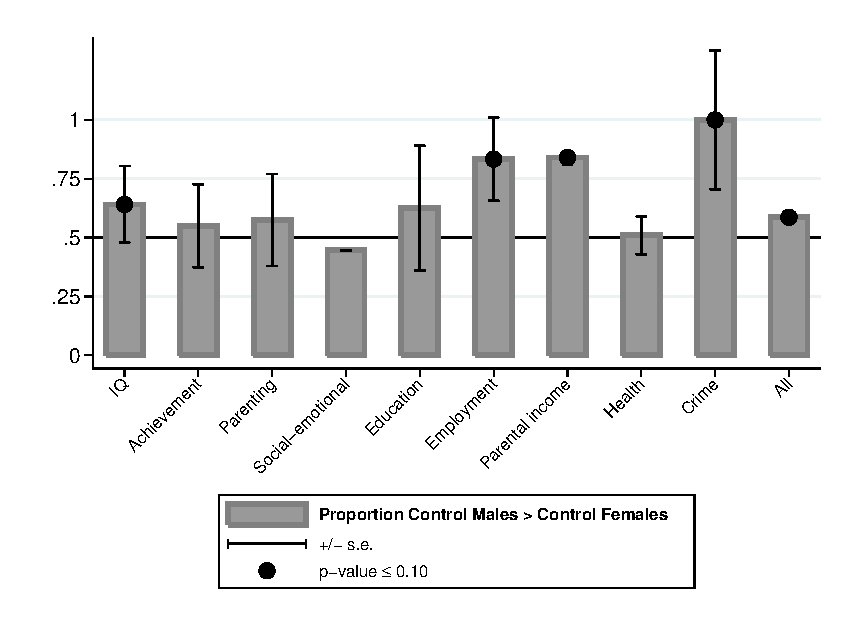
\includegraphics[width=\textwidth]{output/gendergaps-fullcontrol}
\end{subfigure}

\begin{subfigure}[h]{0.8\textwidth}
	\centering
	\caption{Treatment Gender Gaps}
	\label{fig:means-years}
	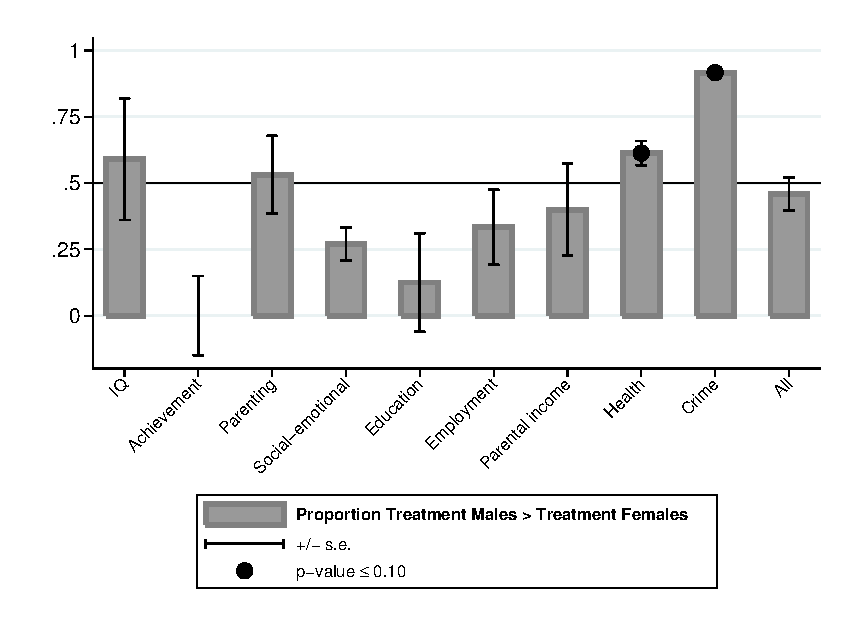
\includegraphics[width=\textwidth]{output/gendergaps-treatment}
\end{subfigure} 
\footnotesize \justify
Note: These plots show the proportion of outcomes, by outcome category, for which the males' mean is larger than the females' mean. The standard errors and the $p$-values are computed using 100 bootstraps. The $p$-values are one-sided and test the null hypothesis that the proportion of outcomes is greater than $\frac{1}{2}$ The crime outcomes are all coded so that a higher value indicates more criminal activity. All other outcome categories have higher values corresponding to socially desirable outcomes. 
\end{figure}

Table~\ref{tab:proportion-table} summarizes the gender gaps in these plots as well as those when considering the alternative setting of the control-group children. In the control group, the proportions of outcomes for which males do better than females is higher than $\frac{1}{2}$ for most of the categories, although by no means are all statistically significant. Exceptions include social-emotional skills, in which females surpass males, and crime, in which the outcomes are coded such that higher values correspond with less criminal activity. \textbf{[JJH: Code crime a positive!]} Treatment reverses the gaps for achievement, education, employment, parental income, and over all outcomes. It widens the gap for health, with treatment leading males to achieve better health outcomes. Considering control-group subjects who stay at home, females have better health outcomes and commit more crimes. Both outcomes are reduced with treatment \textbf{[JJH: Why worse health?]}. Finally, the males who attend lower-quality alternative preschools do not outperform females on any of the outcome categories associated with cognition, education, and parenting. This indicates an early-life disadvantage that enriched early childcare programs partially correct.

\begin{table}[H]
\centering
\caption{Summary of Proportion of Outcomes Males $>$ Females}
\label{tab:proportion-table}
\begin{threeparttable}
\begin{tabular}{l | c |c |c| c}
\toprule
& (1) & (2) & (3) & (4) \\
Category & Control Group  &  Control Group &  Control Group &  Treatment \\
	&				&	Stay at Home		& Alternative Preschool &  Group \\
\midrule  
IQ 								& \checkmark 	&  \checkmark* 		& $\times$	& \checkmark \\
Achievement						& \checkmark* 	&  \checkmark* 		&$\times$		& $\times$* \\
Social-emotional					& $\times$	& \checkmark 		&$\times$* 	&$\times$ \\
Parenting							& \checkmark	&  \checkmark* 		&$\times$ 	& $\times$ \\
Parental income					&  \checkmark  &\checkmark* 		& $\times$  	& \checkmark \\
Education							& \checkmark 	&\checkmark 		& $\times$ 	&	$\times$* \\
Employment						&  \checkmark* &  \checkmark* 		& $=$ 		&\checkmark* \\
Crime							&  $\times$* 	&  $=$ 			& $\times$* 	&  $\times$* \\
Risky Behavior						& $\times$	& $\times$*		& \checkmark	& $\times$* \\
Health 							& $=$ 		& $\times$ 		& $\times$ 	&  \checkmark *\\
Mental Health						& \checkmark* & \checkmark* 		&	\checkmark &	\checkmark \\

\midrule
All								&  \checkmark &\checkmark*&  $\times$ & $\times$\\
\bottomrule
\end{tabular}
\begin{tablenotes}
\footnotesize
\item Note: This table summarizes comparison of gender gaps across outcome categories by different groups. A checkmark indicates that the proportion of outcomes in the corresponding category is larger than $\frac{1}{2}$, meaning that males outperform females. A checkmark with an asterisk indicates that the proportion is significantly larger than $\frac{1}{2}$. Column (1) is the difference between males and females in the full control group.  Column (2) is the difference between males and females in the control group only considering those who stayed at home. Column (3) is the difference between males and females in the control group only considering those who attended alternative preschools. Column (4) is the difference between males and females in the treatment group.
\end{tablenotes}
\end{threeparttable}
\end{table}

Many studies have shown the potential for early-life interventions to improve the skills of children, especially those from disadvantaged families.\footnote{\citet{Currie_2011_AER,Elango_Hojman_etal_2016_Early-Edu}.} Several of these studies report effects by gender and find that males and females differently benefit from early childhood education. For example, \citet{Heckman_Moon_etal_2010_QE} and \citet{Garcia_Heckman_Leaf_etal_2017_Comp_CBA_Unpublished}, analyze randomized controlled trials with long-term data follow-ups, and find that intervening early in life more positively affects education for females and labor market and health outcomes for males. Other studies analyzing programs with shorter-term follow-up also find similar patterns of gender differences in early skills and academic outcomes.\footnote{\citet{Deming_2009_AEJAE,Ou_Reynolds_2010_Mechanisms_CYSR,Magnuson_Kelchen_Duncan_etal_2016_ECRQ}.} None of these studies have examined the gender gap and how treatment alters it.

This paper reports the treatment effects of ABC/CARE by gender. We report treatment effects comparing treated outcomes with different control conditions, including staying at home or attending other center-based care that was of lower quality than the ABC/CARE program.\footnote{Historical documentation, records, and evidence from knowledgeable individuals indicate that although these alternate centers followed state and federal standards, they were of lower quality than the ABC/CARE program.} Unlike previous studies, we compute treatment effects comparing the treatment group to the control group fixing those in the control group to these two alternate counterfactuals (shown in Figure 1?).\footnote{Previous studies presenting treatment effects of ABC and CARE include \citet{Ramey_etal_1985_Project-CARE_TiECSE, Clarke_Campbell_1998_ABC_Comparison_ECRQ,Campbell_Pungello_etal_2001_DP,Campbell_Ramey_etal_2002_ADS,Campbell_Wasik_etal_2008_ECRQ,Campbell_Conti_etal_2014_EarlyChildhoodInvestments}.}$^,$\footnote{See \cite{Heckman_1992_randomization}, \cite{Heckman_Hohmann_etal_2000_QJE}, and \cite{Kline_Walters_2016_QJE} for work related to control substitution.} Home care is beneficial for boys. 

This paper unfolds in the following way. In Section~\ref{sec:data}, we describe the experimental data and its special features. We document that a considerable proportion of the control group children attend lower (than treatment) preschools. In Sections~\ref{sec:parameters} and~\ref{sec:combining-functions} we define the treatment effects estimated. Section~\ref{sec:treatment-effects} reports the treatment effects overall and by gender and establish the existence of sharp gender effects in many categories of outcomes. Section~\ref{sec:gender-differences} discusses differences in the proportions of outcomes favoring men by category. Section~\ref{sec:conclusion} discusses the sources of these differences.


%ee \citet{Beeghly-etal_2017_IMHJ,Dayton_2017_IMHJ,Iruka_2017_IMHJ,Schore_2017_IMHJ} for recent findings on the topic of different development of males and females early in life. 	

\section{Data}
\label{sec:data}
We analyze a combined sample of the two closely related interventions. Table~\ref{tab:abc-care-characteristics} summarizes the characteristics of the programs. Both interventions were implemented by researchers at the Frank Porter Graham Center at the University of North Carolina, Chapel Hill. ABC had four cohorts of subjects born between 1972 and 1977, and CARE had two cohorts of subjects born between 1978 and 1980. Both interventions targeted children from disadvantaged families in the Chapel Hill area. Eligibility was determined based on a High Risk Index (HRI) developed for ABC and minimally adapted for CARE.\footnote{See \citet{Campbell_Wasik_etal_2008_ECRQ}.} Example components of the HRI include father's presence, parental employment, and welfare receipt.\footnote{See Appendix~\ref{appendix:background} for the full HRI. \citet{Ramey_Smith_1977_AJMD, Wasik_Ramey_etal_1990_CD, Ramey_Campbell_1991_childreninpoverty}.}

Both interventions involved intensive center-based care for subjects in the treatment group starting at 8 weeks and continuing until age 5 before the children started kindergarten. Treatment-group subjects also received daily health screenings and diapers and formula until 6 months. Control-group families received the diapers and formula as well for the same period of time.\footnote{\citet{Wasik_Ramey_etal_1990_CD}.}  After school entrance up until age 8, there was an additional component of treatment in which home visitors worked with children and their parents to tutor the children and to encourage families to be involved in the children's academics.\footnote{In ABC, treatment status of this component was randomized. In CARE, all the subjects who received center-based care also received this school-age component.} We do not consider this part of the treatment because it extends beyond early childhood and in other work it was not found to have significant treatment effects.\footnote{\citet{Campbell_Ramey_etal_2002_ADS}.}

The pedagogical approach focused on language, cognitive, social-emotional, and executive functioning skills. During ABC and CARE, the \textit{Learning Games} curriculum was developed and refined.\footnote{\citet{Sparling_Lewis_1979_BOOKLearninggamesFirstThree}.} ABC and CARE subjects engaged with this in addition to other curricula that emphasized child-led learning of skills important for future learning.\footnote{\citet{Conti_etal_2016_LongTermHealth}.}

CARE included an additional arm of treatment. In addition to the services listed above, those in the treatment group received home visiting from birth to age 5. This home visiting consisted of biweekly visits focusing on parental problem solving skills. There was an additional experimental group that received this home visiting component, but not the center-based care.\footnote{\citet{Wasik_Ramey_etal_1990_CD}.} In light of previous analyses, we do not include this last group in our analysis. The home visiting component had weak effects.\footnote{\citet{Campbell_Conti_etal_2014_EarlyChildhoodInvestments} test for pooling.} We also use this lack of treatment effects to justify merging the treatment groups of ABC and CARE, even though that of CARE received the additional home-visiting component.\footnote{\citet{ABCCARE_Dataset}.}

\begin{table}[H]
\centering
\caption{ABC and CARE Program Overview}
\label{tab:abc-care-characteristics}
\begin{threeparttable}
	\begin{tabular}{l l}
	\toprule
Site & Chapel Hill, North Carolina \\
Cohorts & 4 (ABC), 2 (CARE) \\
$N$ & 58 treatment, 56 control (ABC) \\
	& 17 treatment, 23 control (CARE) \\
\midrule
Eligibility & HRI $>$ 11 \\
		& Biologically healthy \\
\midrule
Treatment years & 1972--1981 (ABC), 1977--1983 (CARE) \\
Treatment duration & 5 years \\
\midrule
Home visits 	& 2.5--2.7	per month (CARE)	\\
Center care	& 50	weeks per year \\
		 	& 30--45 hours per week  \\
Other treatment components & Formula until 6 months\\
					& Diapers until 6 months \\ 
					& Health check-ups \\
					& Medical care \\
					& Parenting instruction \\
					& Counseling \\
					& Transportation to center \\
Control-group incentives & Formula until 6 months \\
				& Diapers until 6 months 	\\
				& Health check-ups until 1 year (ABC, cohort 1) \\
\midrule
Adult-child ratio & 1:3--1:6 \\
Teacher requirements & High school through masters \\
				& Experience with children \\
Specialists & Physician, nurse, social worker \\
\bottomrule
\end{tabular}



\begin{tablenotes}
\footnotesize
\item Note: Characteristics that do not specify ABC or CARE were present in both. Biologically healthy includes lack of serious illness, including mental retardation. \\
\item Sources: \citet{Ramey_Collier_etal_1976_CarolinaAbecedarianProject,Ramey_Smith_1977_AJMD,Ramey_etal_1985_Project-CARE_TiECSE,Wasik_Ramey_etal_1990_CD,Ramey_Campbell_1991_childreninpoverty}.
\end{tablenotes}
\end{threeparttable}
\end{table}

Figure~\ref{fig:family-over-time} presents one aspect of family disadvantage.  The figure shows the evolution of the fathers' presence over time. At birth, there were few fathers present, especially for the females in the treatment group. This is a pattern commonly found in the literature. After birth, the proportion of fathers present, conditional being present at birth, remains stable.\footnote{For a more detailed description of the sample's disadvantage, see Appendix~\ref{appendix:background}.}

\begin{figure}[H]
\textbf{[JJH: Looks like a treatment effect on father present.][We report treatment effects on father present in Appendix C. There is a negative treatment effect for females between 3 and 5 years.}
\begin{center}
\caption{Father Present Over Time}
\label{fig:family-over-time}
		\label{fig:fhome}
			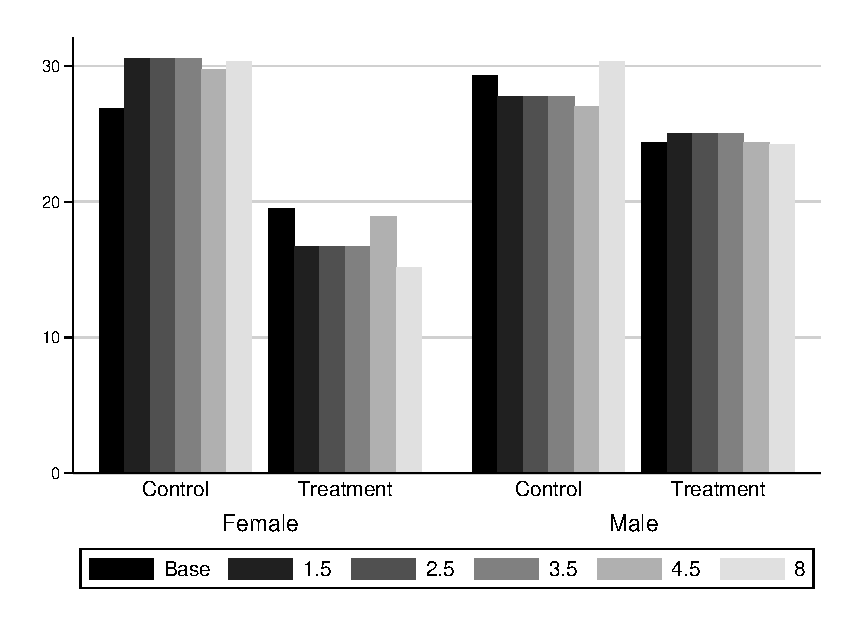
\includegraphics[width=0.65\textwidth]{output/family-fhome}
\end{center}
\footnotesize \justify
Note: The bars represent the proportion of father's presence. The bars after baseline are conditional on the father being at home at baseline.
\end{figure}

\subsection{Randomization Protocol and Compromises} \label{section:randomization}

Randomization for ABC/CARE was conducted on child pairs matched on family background. Siblings and twins were jointly randomized into either treatment or control groups.\footnote{For siblings, this occurred when two siblings were close enough in age such that both of them were eligible for the program.} Randomization pairing was based on a risk index, maternal education, maternal age, and gender of the subject.\footnote{We do not know the original pairs.} ABC collected an initial sample of 121 subjects. We characterize each missing observation in Appendix~\ref{appendix:background}.\footnote{In Appendix~\ref{appendix:estimates}, we document that our estimates are robust when we adjust for missing data using standard weighting (matching) methods described in Appendix~\ref{app:method_partialobs}.} We conduct the same analysis for the CARE sample. 22 subjects in ABC did not stay in the program through age 5. Dropouts are evenly balanced and are primarily related to the health of the child and mobility of families and not to dissatisfaction with the program.\footnote{The 22 dropouts include four children who died, four children who left the study because their parents moved, and two children who were diagnosed as developmentally delayed. Details are in Table~\ref{table:abccompromises}. Everyone offered the program was randomized to either treatment or control. All eligible families agreed to participate. Dropping out occurs \emph{after} randomization.}

\subsection{Control Group Substitution}

In ABC/CARE, many control-group subjects (but no treatment-group subjects) attended alternative center-based preschool.\footnote{See \cite{Heckman_Hohmann_etal_2000_QJE} on the issue of substitution bias in social experiments.} The figure is \treatsubsabc\ for ABC and \treatsubscarec\ for CARE. This creates both a problem (substitution bias\footnote{See \cite{Heckman_1992_randomization}, \cite{Heckman_Hohmann_etal_2000_QJE}, and \cite{Kline_Walters_2016_QJE}.}) and an opportunity (we can compare the effect of an enriched treatment vs. other alternative home and low quality environments). We discuss both.

\begin{sidewaysfigure}[!htbp]
\centering
\caption{Control Substitution Characteristics, ABC/CARE Control Group}\label{fig:control-sub}
\begin{subfigure}[h]{0.49\textwidth}
	\centering
	\caption{Cumulative Enrollment} \label{fig:treatsubcare}
	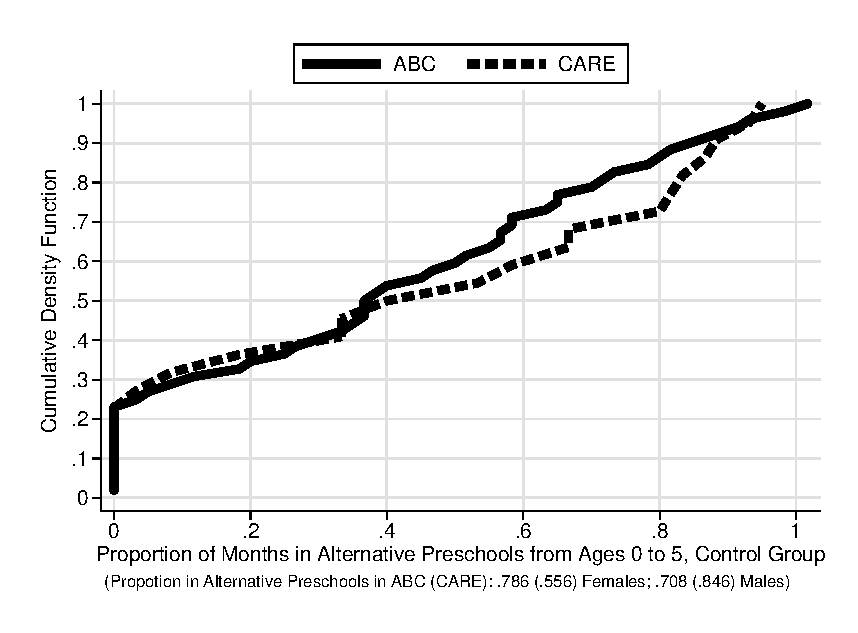
\includegraphics[width=\textwidth]{output/abccare_controlcontamination.eps}
\end{subfigure}
\begin{subfigure}[h]{0.49\textwidth}
	\centering
	\caption{Enrollment Dynamics} \label{fig:proportion-alt-pre}
	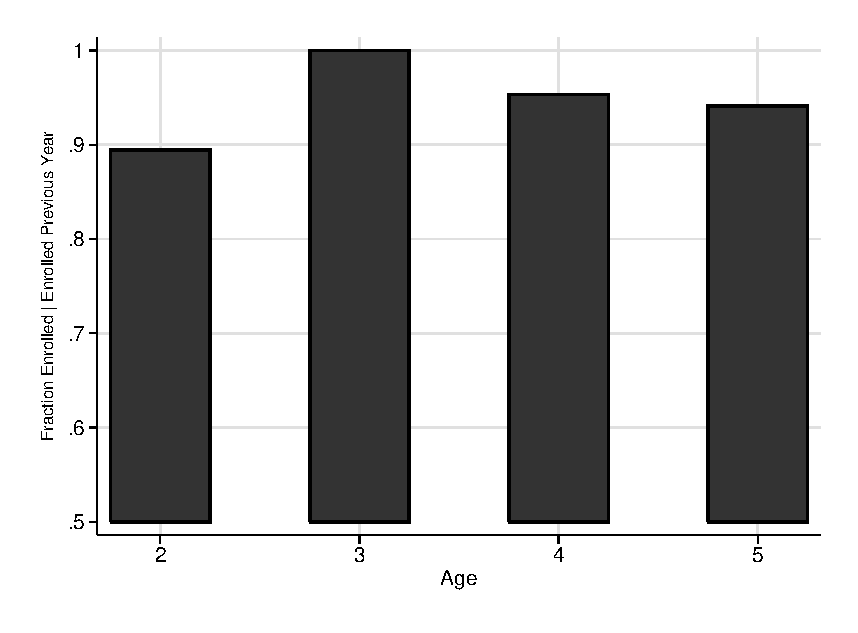
\includegraphics[width=\textwidth]{output/abccare_Vprobs.eps}
\end{subfigure}%
\footnotesize \justify
Note: Panel (a) displays the cumulative distribution function of enrollment in alternatives. Panel (b) displays the fraction of ABC/CARE control-group children enrolled in alternatives, conditional on being enrolled in the previous age (at least one month).\\
\end{sidewaysfigure}

Figure~\ref{fig:treatsubcare} shows the cumulative distribution of the proportion of time in the first five years that control subjects were enrolled in alternatives. Figure~\ref{fig:proportion-alt-pre} shows the dynamics of enrollment. Those who enroll generally stay enrolled. As control children age, they are more likely to enter childcare (see Appendix~\ref{app:control-subbb}).

Children in the control group who are enrolled in alternative early childcare programs are less economically disadvantaged at baseline compared to children who stay at home. Disadvantage is measured by maternal education, maternal IQ, Apgar scores, and the high-risk index defining ABC/CARE eligibility. Children who attend alternatives have fewer siblings. On average, they are children of mothers who are more likely to be working at baseline.\footnote{Statistically significant at 10\%.} Parents of girls are much more likely to use alternative childcare if assigned to the control group.\footnote{See Table~\ref{table:controlsubscharacteristics} in Appendix~\ref{appendix:background} for tests of differences across these variables between children in the control group who attended and who did not attend alternative preschools.} If a boy, father more likely present.

While most of the alternative childcare centers received federal subsidies and were subject to the federal regulations of the era, they were relatively low quality compared to ABC/CARE.\footnote{Appendix~\ref{appendix:tetanus} discusses the federal standards of that day. See \citet{Department-of-Health_1968_DayCareRequirements,NCGA_1971_House-Bill-100,Ramey-et-al_1977_Intro-to-ABC,Ramey_Campbell_1979_SR,Ramey_McGinness_etal_1982_Abecedarianapproach, Burchinal_Campbell_etal_1997_CD}.}$^,$\footnote{When we compare ABC/CARE treatment to these alternatives, ABC/CARE has substantial treatment effects. Further, as we argue below, parents perceived that ABC/CARE was superior to the alternatives.} The access of control-group children to alternative programs affects the interpretation of estimated treatment effects, as we discuss next.


\section{Parameters of Interest}
\label{sec:parameters}
Random assignment to treatment does not guarantee that conventional treatment effect estimators answer policy-relevant questions. We define and estimate three parameters that address different policy questions.

Let $W=1$ indicate that the parents referred to the program participate in the randomization protocol. $W=0$ indicates otherwise. $R$ indicates randomization into the treatment group ($R = 1$) or to the control group ($R = 0$). $D$ indicates attending the program, i.e., $D = R$ implies compliance with the initial randomization protocol.

Individuals are eligible to participate in the program if baseline background variables $\bm{B}\in\mathcal{B}_0$. $\mathcal{B}_0$ is the set of scores on the risk index that determines program eligibility. Because all of the eligible people given the option to participate choose to do so $(W=1\text{ and } D=R)$, we can safely interpret the treatment effects generated by the experiment as average treatment effects for the population for which $\bm{B}\in\mathcal{B}_0$ and not just treatment effects for the treated.\footnote{According to \citet{Ramey_Yeates_Short_1984_CD}, there was only one eligible mother who refused to participate in the randomization.}

Let $Y^1_{j}$ be the outcome $j$ for the treated, and $Y^0_{j}$ be the control counterfactual. $Y^0_{j}$ depends on the exposure to various alternative preschools while ABC/CARE was active (i.e.,\ it depends on the degree of control substitution).\footnote{This is an example of control-group subjects of a social experiment finding a treatment substitute. See \cite{Heckman_Hohmann_etal_2000_QJE} for methodological solutions and an example of implementation.} The index set for the outcomes is $\mathcal{J}$, which we can partition by age (\ $\mathcal{J}_a$ with $\mathcal{J} = \bigcup \limits _{a \in \mathcal{A}} \mathcal{J}_a$ and $\mathcal{A}$ indexes age) or by outcome category (\ $\mathcal{J}_\ell$ with $\mathcal{J} = \bigcup \limits _{\ell \in \mathcal{L}} \mathcal{J}_\ell$ and $\mathcal{L}$ indexes categories).

All treatment-group children had the same exposure to the ABC/CARE treatment and no exposure to alternative center-based care.\footnote{We discuss cases of attrition during the program in Appendix~\ref{appendix:background}.} It would be desirable to identify and estimate parameters evaluating ABC/CARE against all possible levels of exposure to alternative preschools, but our samples are too small to credibly do so. We simplify the analysis of the counterfactual to ABC/CARE by creating two categories. ``$H$'' indicates that the control-group child stays at home throughout the entire length of the program. ``$C$'' indicates that a control-group child is in alternative center childcare for any amount of time.\footnote{This categorization is consistent with Figure~\ref{fig:proportion-alt-pre}. Once parents decided to enroll their children in alternative preschools, the children tended to stay enrolled up to age 5.} We test the sensitivity of our estimates to the choice of different categorizations in our empirical analysis in Appendix~\ref{appendix:vsensitivity-controlsub}. We thus compress a complex reality into two counterfactual outcome states for each outcome $j$:
\begin{align*}
Y_{j,H}^0 \quad &: \quad \textbf{ Subject received home care exclusively} \\
Y_{j,C}^0 \quad &: \quad \textbf{ Subject attended some alternative preschool}.
\end{align*}


One parameter of interest addresses the question: What is the effect of the program as implemented? This is the effect of the program compared to the next best alternative as perceived by the parents (or the relevant decision maker) and is defined by
\begin{equation}\label{eq:effect}
\Delta_j := \mathbb{E} \left[ Y_{j}^1 -  Y_{j}^0 | W =1 \right] = \mathbb{E} \left[Y_{j}^1 -  Y_{j}^0 | \bm{B} \in \mathcal{B}_0 \right],
\end{equation}
where the second equality follows because everyone who was eligible elected to participate in the program. For the sample of eligible people, this parameter addresses the effectiveness of the program relative to the quality of all available alternatives when the program was implemented, including staying at home. This is the Local Average Treatment Effect (LATE).\footnote{\citet{Imbens_Angrist_1994_Econometrica}.}

We define $V$ as a dummy variable indicating that the control-group child attended alternative center-based childcare. $V=0$ denotes that the control-group child stayed at home. The outcome when a child is in the control group is
\begin{equation}
Y_{j}^0 : = \left( 1 - V \right) Y_{j,H}^0 + \left( V \right) Y_{j,C}^0. \label{eq:meandiff}
\end{equation}
\noindent It is fruitful to assess the effectiveness of the program compared to a world in which the child stays at home full time. The associated causal parameter is:
\begin{equation}\label{eq:cont1}
\Delta_j \left(\text{\textbf{Fix }}V = 0 \right) : =   \mathbb{E} \left[ Y_{j}^1 -  Y_{j}^0 | \text{\textbf{Fix }}V = 0, W = 1 \right] := \mathbb{E} \left[Y_{j}^1 -  Y_{j}^0 | \text{\textbf{Fix }}V = 0, \bm{B} \in \mathcal{B}_0 \right].
\end{equation}
It is also useful to assess the average effectiveness of a program relative to attending an alternative preschool with associated causal parameter:
\begin{equation}\label{eq:cont2}
\Delta_j \left( \text{\textbf{Fix }} V =1 \right) : =   \mathbb{E} \left[ Y_{j}^1 -  Y_{j}^0 | \text{\textbf{Fix }} V = 1, W = 1 \right] := \mathbb{E} \left[ Y_{j}^1 -  Y_{j}^0 | \text{\textbf{Fix }} V = 1, \bm{B} \in \mathcal{B}_0 \right].
\end{equation}

\noindent ``\textbf{Fix}'' means $V$ is fixed to the designated value.\footnote{For the distinction between fixing and conditioning, see \citet{Haavelmo_1943_Econometrica} and \citet{Heckman_Pinto_2015_EconometTheory}.}

Random assignment to treatment does not directly identify the parameters in Equations~\eqref{eq:cont1} or~\eqref{eq:cont2}. Econometric methods are required. In this paper, we rely on matching to control for selection into home or an alternative preschool by the control group. We assume that observed characteristics are sufficient to describe the selection into alternative center-based arrangements. In Appendix~\ref{appendix:results}, we show the balance across the groups in the matched samples along the observed selection variables (e.g., family characteristics, Apgar scores, gender), further justifying this approach.\footnote{To select adequate variables for matching, we conduct goodness of fit tests to find the most predictive set of baseline characteristics subject to penalty for adding parameters. This procedure is fully explained in Appendix~\ref{appendix:results}.}

We report estimates from alternative empirical strategies, including instrumental variables and control functions, in Appendix~\ref{appendix:amethodology}. The estimates from these alternative estimation strategies are consistent with results from matching but lack precision. Appendix~\ref{appendix:vsensitivity-controlsub} displays results with alternative definitions of $V$ (i.e., different thresholds define if a child attended alternative preschool). The results are robust to the various definitions. What matters is whether any center-based child care is being used ($V>0$)---not the specific value of $V$.

\subsection{Summarizing Multiple Treatment Effects}\label{sec:combining-functions}

The extensive data for ABC/CARE generates many outcomes that we can use to evaluate the program. Summarizing these effects in an interpretable way is challenging.\footnote{In Appendix~\ref{appendix:results} we present an exhaustive list of treatment effects correcting the $p$-values using the step-down procedure in \citet{Romano_Wolf_2016_pval_SaPL}.} We present effect sizes averaged over outcomes. We also construct combining functions that count the proportion of treatment effects that are positive for different categories of outcomes. Similarly, we study the count of the proportion of treatment effects that are positive and statistically significant at the 10\% level. We complement these analyses by applying an exact non-parametric test on the equality of the distributions of outcomes across treatment groups developed in \citet{Rosenbaum_2005_Distribution_JRSS}.

\textbf{Combining Functions.} Consider a block of outcomes $\mathcal{J}_{\ell}, \ell \in \{1,\dots ,L\}$, with cardinality $B_{\ell}$ and  associated treatment effects $\Delta_1, \ldots \Delta_{B_\ell}$. We assume that outcomes can be ordered so that $\Delta_{j} >0$ is beneficial.\footnote{All but 5\% of the outcomes we study can be ranked in this fashion. See Appendix~\ref{appendix:results} for a discussion.} The count of positive treatment effects within block $\mathcal{J}_{\ell}$ is:
\begin{equation}
C_\ell = \sum^{B_\ell}_{j=1} \bm{1} (\Delta_{j} >0),
\end{equation}

\noindent The proportion of beneficial outcomes, our combining function, is $C_\ell / B_\ell$. In our empirical application we consider all the outcomes as a block. Different blocks are grouped by age (e.g.,\ childhood, school age, adulthood) or by common categories (e.g.,\ employment, health, crime).

Under the null hypothesis of no treatment effect for the block of outcomes indexed by $\mathcal{J}_\ell$, and assuming the validity of asymptotic approximations, $C_\ell / B_\ell$ is centered at $\frac{1}{2}$.\footnote{\citet{Campbell_Conti_etal_2014_EarlyChildhoodInvestments} establish a validity of asymptotic approximations for the ABC sample.} We compute the fraction $C_\ell / B_\ell$ and the corresponding bootstrapped empirical distribution to obtain a $p$-value. The bootstrap procedure accounts for dependence in unobservables across outcomes (within blocks) in a general way.

Our test based on the number of outcomes for which the treatment effect is statistically significant at the $10\%$ level produces similar inference. Under the null hypothesis, 10\% of all outcomes should be ``significant'' at the 10\% level even if there is no treatment effect of the program.\footnote{In this case, we perform a ``double bootstrap'' procedure to first determine significant treatment effects at $10\%$ level and then calculate the standard error of the count.} The combining functions avoid: (i) arbitrarily picking outcomes that have statistically significant effects---``cherry picking''; or (ii) arbitrarily selecting blocks of outcomes to correct the $p$-values when accounting for multiple hypothesis testing. We present $p$-values for these hypotheses and a number of combining functions by outcome category in Appendix~\ref{appendix:results}.\footnote{In Appendix~\ref{appendix:results}, we present yet another alternative. We calculate a latent measure, using principal component analysis, of the set of outcomes within a block and perform inference on this latent measure. This analysis also points to beneficial effects of the program.}

\textbf{An Exact Non-Parametric Test.} We also test for equality of treatment and control distributions by outcome using an exact test developed by \citet{Rosenbaum_2005_Distribution_JRSS}. We provide a brief explanation of the test and refer interested readers to the original source for more details. Let $\mathcal{N}$ index the individuals in our sample and consider the block of outcomes $\mathcal{J}_\ell$. Let $d_{ii'}$ be the distance between the individuals $i, i' \in \mathcal{N}$, $i \neq i'$, based on the outcomes in $\mathcal{J}_\ell$. In our application, this is the Mahalanobis distance.\footnote{\citet{Mahalanobis_1936_PNISI}.} There is an optimal non-bipartite pairing of individuals according to $d_{ii'}$.\footnote{\citet{Derigs_1988_Solving_AOR}.} This is obtained by minimizing the distance across all possible pairings $i, i'$ in the sample.

Under the null hypothesis of no treatment effects, pairings of treatment-group children with control-group children should be as frequent as pairings of treatment-group children with other treatment-group children and control-group children with other control-group children. If a relatively large number of pairs are matched equally across groups using this metric, we fail to reject the null hypothesis that the joint distribution of outcomes in block $\mathcal{J}_{\ell}, \ell \in \{1,\dots ,L\}$ is the same across the treatment and control groups.

The number of treatment-control pairings in the optimal non-bipartite pairing within the block of outcomes $\mathcal{J}_\ell$, denoted by $A_{\ell}, \ell \in \{1,\dots ,L\}$, is a summary statistic allowing us to test the null hypothesis of interest. Its exact $p$-value can be calculated. Asymptotically, the studentized value of $A_\ell$ follows a normal standard distribution. For each block, we present these asymptotic $p$-values to complement the information provided by the combining functions.\footnote{The exact $p$-values render similar results. We display the asymptotic $p$-values for expositional simplicity.}


\section{Estimates and Tests of Differences in Treatment Effects}
\label{sec:treatment-effects}
This section reports estimates of treatment effects for the main outcomes by gender, tests of equality of effects by outcome, and the estimated combining functions. These estimates show that the program treatment effects are strong for both males and females are that treatment effects depend on the counterfactual against which they are benchmarked (home or low quality center care). Treatment effects sharply differ by gender.

\subsection{Estimated Treatment Effects}

Tables~\ref{table:tescombinedmales} and \ref{table:tescombinedfemales} present the estimates of a representative selection of the main treatment effects for males and females respectively. The full list of treatment effects is reported in Web Appendix~\ref{appendix:results}. Column (1) of each table gives sample mean differences in outcomes between treatment and control groups. Column (2) adjusts the differences for attrition and controls for background variables. Both are estimates of the parameter defined in equation~\eqref{eq:effect}, but with different conditioning sets. Column (3) shows the mean difference between the full treatment-group and the control-group subjects who did not attend alternative preschools. Column (4) gives standard matching estimates for the parameter defined in equation~\eqref{eq:influenza}.\footnote{In Appendix~\ref{app:matching-is-fun}, we provide details on: (i) the kernel matching estimator that we use; (ii) the matching variables that we use; and (iii) a sensitivity analysis to these matching variables.} Column (5) reports estimates of the parameter defined by equation~\eqref{eq:smallpox}. mean differences between the full treatment-group and control-group children who attended alternatives. Column (6) gives matching estimates for the parameter of equation~\eqref{eq:smallpox}.

The results for females show that ABC/CARE has substantial effects on education when comparing outcomes of the treatment-group subjects to those from the next best alternative. High school graduation increases between 13 and 25 percentage points, depending on the estimate that we consider; college graduation increases 13 percentage points; and the average years of schooling increase between 2.1 and 1.8 years. Employment at age 30 increases between 13 and 8 percentage points. ABC/CARE has substantial impacts on human capital accumulation and employment. The results strengthen when we compare treatment with the option of staying at home.

\begin{sidewaystable}[!htbp]
\centering
\begin{threeparttable}
\caption{Treatment Effects on Selected Outcomes, Males}\label{table:tescombinedmales}
\begin{scriptsize}
  \begin{tabular}{cccccccccccc}
  \toprule
   Category & Variable & Age & $\bar{Y}_C$ & (1) & (2) & (3) & (4) & (5) & (6) \\

    \midrule
    % cat 3
     \mc{1}{l}{\scriptsize{Parental Income}} &   \mc{1}{l}{\scriptsize{Parental Labor Income}} & \mc{1}{c}{\scriptsize{3.5}} & \mc{1}{c}{\scriptsize{13,505}} & \mc{1}{c}{\scriptsize{1,036}} & \mc{1}{c}{\scriptsize{494}} & \mc{1}{c}{\scriptsize{73.862}} & \mc{1}{c}{\scriptsize{1,462}} & \mc{1}{c}{\scriptsize{123}} & \mc{1}{c}{\scriptsize{690}} \\  

  &   &  & & \mc{1}{c}{\scriptsize{(0.374)}} & \mc{1}{c}{\scriptsize{(0.411)}} & \mc{1}{c}{\scriptsize{(0.474)}} & \mc{1}{c}{\scriptsize{(0.390)}} & \mc{1}{c}{\scriptsize{(0.479)}} & \mc{1}{c}{\scriptsize{(0.417)}} \\  

  &   & \mc{1}{c}{\scriptsize{12}} & \mc{1}{c}{\scriptsize{23,868}} & \mc{1}{c}{\scriptsize{7,085}} & \mc{1}{c}{\scriptsize{9,625}} & \mc{1}{c}{\scriptsize{18,050}} & \mc{1}{c}{\scriptsize{12,639}} & \mc{1}{c}{\scriptsize{6,620}} & \mc{1}{c}{\scriptsize{5,383}} \\  

  &   &  & & \mc{1}{c}{\scriptsize{\textbf{(0.092)}}} & \mc{1}{c}{\scriptsize{\textbf{(0.020)}}} & \mc{1}{c}{\scriptsize{\textbf{(0.038)}}} & \mc{1}{c}{\scriptsize{\textbf{(0.074)}}} & \mc{1}{c}{\scriptsize{\textbf{(0.098)}}} & \mc{1}{c}{\scriptsize{(0.139)}} \\  

  &   & \mc{1}{c}{\scriptsize{15}} & \mc{1}{c}{\scriptsize{22,985}} & \mc{1}{c}{\scriptsize{8,488}} & \mc{1}{c}{\scriptsize{4,495}} & \mc{1}{c}{\scriptsize{5,540}} & \mc{1}{c}{\scriptsize{4,805}} & \mc{1}{c}{\scriptsize{2,885}} & \mc{1}{c}{\scriptsize{4,345}} \\  

  &   &  & & \mc{1}{c}{\scriptsize{\textbf{(0.071)}}} & \mc{1}{c}{\scriptsize{(0.221)}} & \mc{1}{c}{\scriptsize{(0.243)}} & \mc{1}{c}{\scriptsize{(0.264)}} & \mc{1}{c}{\scriptsize{(0.354)}} & \mc{1}{c}{\scriptsize{(0.296)}} \\  

  &   & \mc{1}{c}{\scriptsize{21}} & \mc{1}{c}{\scriptsize{21,585}} & \mc{1}{c}{\scriptsize{12,732}} & \mc{1}{c}{\scriptsize{8,809}} & \mc{1}{c}{\scriptsize{122}} & \mc{1}{c}{\scriptsize{-933}} & \mc{1}{c}{\scriptsize{10,784}} & \mc{1}{c}{\scriptsize{10,283}} \\  

  &   &  & & \mc{1}{c}{\scriptsize{\textbf{(0.005)}}} & \mc{1}{c}{\scriptsize{\textbf{(0.098)}}} & \mc{1}{c}{\scriptsize{(0.448)}} & \mc{1}{c}{\scriptsize{(0.456)}} & \mc{1}{c}{\scriptsize{\textbf{(0.056)}}} & \mc{1}{c}{\scriptsize{\textbf{(0.041)}}} \\  

   \mc{1}{l}{\scriptsize{Education}} &   \mc{1}{l}{\scriptsize{Graduated High School}} & \mc{1}{c}{\scriptsize{30}} & \mc{1}{c}{\scriptsize{0.600}} & \mc{1}{c}{\scriptsize{0.073}} & \mc{1}{c}{\scriptsize{0.044}} & \mc{1}{c}{\scriptsize{0.116}} & \mc{1}{c}{\scriptsize{0.083}} & \mc{1}{c}{\scriptsize{0.040}} & \mc{1}{c}{\scriptsize{0.063}} \\  

  &   &  & & \mc{1}{c}{\scriptsize{(0.262)}} & \mc{1}{c}{\scriptsize{(0.375)}} & \mc{1}{c}{\scriptsize{\textbf{(0.001)}}} & \mc{1}{c}{\scriptsize{(0.346)}} & \mc{1}{c}{\scriptsize{(0.407)}} & \mc{1}{c}{\scriptsize{(0.317)}} \\  

  &  \mc{1}{l}{\scriptsize{Graduated 4-year College}} & \mc{1}{c}{\scriptsize{30}} & \mc{1}{c}{\scriptsize{0.120}} & \mc{1}{c}{\scriptsize{0.170}} & \mc{1}{c}{\scriptsize{0.138}} & \mc{1}{c}{\scriptsize{0.149}} & \mc{1}{c}{\scriptsize{0.099}} & \mc{1}{c}{\scriptsize{0.135}} & \mc{1}{c}{\scriptsize{0.143}} \\  

  &   &  & & \mc{1}{c}{\scriptsize{\textbf{(0.055)}}} & \mc{1}{c}{\scriptsize{(0.128)}} & \mc{1}{c}{\scriptsize{(0.216)}} & \mc{1}{c}{\scriptsize{(0.338)}} & \mc{1}{c}{\scriptsize{(0.154)}} & \mc{1}{c}{\scriptsize{(0.130)}} \\  

  &  \mc{1}{l}{\scriptsize{Years of Education}} & \mc{1}{c}{\scriptsize{30}} & \mc{1}{c}{\scriptsize{12.867}} & \mc{1}{c}{\scriptsize{0.525}} & \mc{1}{c}{\scriptsize{0.541}} & \mc{1}{c}{\scriptsize{1.010}} & \mc{1}{c}{\scriptsize{0.777}} & \mc{1}{c}{\scriptsize{0.351}} & \mc{1}{c}{\scriptsize{0.344}} \\  

  &   &  & & \mc{1}{c}{\scriptsize{(0.151)}} & \mc{1}{c}{\scriptsize{(0.163)}} & \mc{1}{c}{\scriptsize{(0.998)}} & \mc{1}{c}{\scriptsize{(0.136)}} & \mc{1}{c}{\scriptsize{(0.280)}} & \mc{1}{c}{\scriptsize{(0.256)}} \\  

   \mc{1}{l}{\scriptsize{Labor Income}} &   \mc{1}{l}{\scriptsize{Employed}} & \mc{1}{c}{\scriptsize{30}} & \mc{1}{c}{\scriptsize{0.700}} & \mc{1}{c}{\scriptsize{0.119}} & \mc{1}{c}{\scriptsize{0.196}} & \mc{1}{c}{\scriptsize{0.108}} & \mc{1}{c}{\scriptsize{0.040}} & \mc{1}{c}{\scriptsize{0.237}} & \mc{1}{c}{\scriptsize{0.261}} \\  

 &    &  & & \mc{1}{c}{\scriptsize{(0.128)}} & \mc{1}{c}{\scriptsize{\textbf{(0.025)}}} & \mc{1}{c}{\scriptsize{\textbf{(0.001)}}} & \mc{1}{c}{\scriptsize{(0.383)}} & \mc{1}{c}{\scriptsize{\textbf{(0.025)}}} & \mc{1}{c}{\scriptsize{\textbf{(0.013)}}} \\  

  &  \mc{1}{l}{\scriptsize{Labor Income}} & \mc{1}{c}{\scriptsize{30}} & \mc{1}{c}{\scriptsize{30,079}} & \mc{1}{c}{\scriptsize{19,810}} & \mc{1}{c}{\scriptsize{24,365}} & \mc{1}{c}{\scriptsize{25,220}} & \mc{1}{c}{\scriptsize{20,611}} & \mc{1}{c}{\scriptsize{23,072}} & \mc{1}{c}{\scriptsize{21,836}} \\  

   &  &  & & \mc{1}{c}{\scriptsize{\textbf{(0.091)}}} & \mc{1}{c}{\scriptsize{\textbf{(0.092)}}} & \mc{1}{c}{\scriptsize{(0.998)}} & \mc{1}{c}{\scriptsize{(0.122)}} & \mc{1}{c}{\scriptsize{(0.107)}} & \mc{1}{c}{\scriptsize{\textbf{(0.094)}}} \\  

  \mc{1}{l}{\scriptsize{Crime}} &    \mc{1}{l}{\scriptsize{Total Felony Arrests}} & \mc{1}{c}{\scriptsize{Mid-30s}} & \mc{1}{c}{\scriptsize{1.370}} & \mc{1}{c}{\scriptsize{0.196}} & \mc{1}{c}{\scriptsize{0.685}} & \mc{1}{c}{\scriptsize{1.523}} & \mc{1}{c}{\scriptsize{1.340}} & \mc{1}{c}{\scriptsize{0.481}} & \mc{1}{c}{\scriptsize{0.188}} \\  

   &  &  & & \mc{1}{c}{\scriptsize{(0.368)}} & \mc{1}{c}{\scriptsize{(0.183)}} & \mc{1}{c}{\scriptsize{\textbf{(0.064)}}} & \mc{1}{c}{\scriptsize{\textbf{(0.026)}}} & \mc{1}{c}{\scriptsize{(0.284)}} & \mc{1}{c}{\scriptsize{(0.410)}} \\  

  &  \mc{1}{l}{\scriptsize{Total Misdemeanor Arrests}} & \mc{1}{c}{\scriptsize{Mid-30s}} & \mc{1}{c}{\scriptsize{1.296}} & \mc{1}{c}{\scriptsize{-0.501}} & \mc{1}{c}{\scriptsize{-0.244}} & \mc{1}{c}{\scriptsize{-0.298}} & \mc{1}{c}{\scriptsize{-0.034}} & \mc{1}{c}{\scriptsize{-0.246}} & \mc{1}{c}{\scriptsize{-0.507}} \\  

  &   &  & & \mc{1}{c}{\scriptsize{(0.171)}} & \mc{1}{c}{\scriptsize{(0.289)}} & \mc{1}{c}{\scriptsize{(0.314)}} & \mc{1}{c}{\scriptsize{(0.422)}} & \mc{1}{c}{\scriptsize{(0.329)}} & \mc{1}{c}{\scriptsize{(0.168)}} \\  

   \mc{1}{l}{\scriptsize{Health}} &   \mc{1}{l}{\scriptsize{Self-reported drug user}} & \mc{1}{c}{\scriptsize{Mid-30s}} & \mc{1}{c}{\scriptsize{0.500}} & \mc{1}{c}{\scriptsize{-0.333}} & \mc{1}{c}{\scriptsize{-0.438}} & \mc{1}{c}{\scriptsize{-0.673}} & \mc{1}{c}{\scriptsize{-0.557}} & \mc{1}{c}{\scriptsize{-0.326}} & \mc{1}{c}{\scriptsize{-0.330}} \\  

   &  &  & & \mc{1}{c}{\scriptsize{\textbf{(0.019)}}} & \mc{1}{c}{\scriptsize{\textbf{(0.002)}}} & \mc{1}{c}{\scriptsize{\textbf{(0.000)}}} & \mc{1}{c}{\scriptsize{\textbf{(0.000)}}} & \mc{1}{c}{\scriptsize{\textbf{(0.039)}}} & \mc{1}{c}{\scriptsize{\textbf{(0.023)}}} \\  

  &  \mc{1}{l}{\scriptsize{Systolic Blood Pressure (mm Hg)}} & \mc{1}{c}{\scriptsize{Mid-30s}} & \mc{1}{c}{\scriptsize{138.071}} & \mc{1}{c}{\scriptsize{-9.791}} & \mc{1}{c}{\scriptsize{-13.275}} & \mc{1}{c}{\scriptsize{14.196}} & \mc{1}{c}{\scriptsize{14.976}} & \mc{1}{c}{\scriptsize{-24.166}} & \mc{1}{c}{\scriptsize{-18.559}} \\  

  &   &  & & \mc{1}{c}{\scriptsize{(0.113)}} & \mc{1}{c}{\scriptsize{\textbf{(0.049)}}} & \mc{1}{c}{\scriptsize{\textbf{(0.013)}}} & \mc{1}{c}{\scriptsize{\textbf{(0.000)}}} & \mc{1}{c}{\scriptsize{\textbf{(0.000)}}} & \mc{1}{c}{\scriptsize{\textbf{(0.011)}}} \\  

  &  \mc{1}{l}{\scriptsize{Diastolic Blood Pressure (mm Hg)}} & \mc{1}{c}{\scriptsize{Mid-30s}} & \mc{1}{c}{\scriptsize{89.214}} & \mc{1}{c}{\scriptsize{-10.854}} & \mc{1}{c}{\scriptsize{-14.134}} & \mc{1}{c}{\scriptsize{-9.709}} & \mc{1}{c}{\scriptsize{-8.741}} & \mc{1}{c}{\scriptsize{-18.387}} & \mc{1}{c}{\scriptsize{-13.987}} \\  

  &   &  & & \mc{1}{c}{\scriptsize{\textbf{(0.032)}}} & \mc{1}{c}{\scriptsize{\textbf{(0.004)}}} & \mc{1}{c}{\scriptsize{\textbf{(0.049)}}} & \mc{1}{c}{\scriptsize{\textbf{(0.032)}}} & \mc{1}{c}{\scriptsize{\textbf{(0.000)}}} & \mc{1}{c}{\scriptsize{\textbf{(0.007)}}} \\  

  &  \mc{1}{l}{\scriptsize{Hypertension}} & \mc{1}{c}{\scriptsize{Mid-30s}} & \mc{1}{c}{\scriptsize{0.571}} & \mc{1}{c}{\scriptsize{-0.291}} & \mc{1}{c}{\scriptsize{-0.377}} & \mc{1}{c}{\scriptsize{-0.120}} & \mc{1}{c}{\scriptsize{-0.074}} & \mc{1}{c}{\scriptsize{-0.492}} & \mc{1}{c}{\scriptsize{-0.434}} \\  

   &  &  & & \mc{1}{c}{\scriptsize{\textbf{(0.042)}}} & \mc{1}{c}{\scriptsize{\textbf{(0.009)}}} & \mc{1}{c}{\scriptsize{(0.302)}} & \mc{1}{c}{\scriptsize{(0.353)}} & \mc{1}{c}{\scriptsize{\textbf{(0.006)}}} & \mc{1}{c}{\scriptsize{\textbf{(0.006)}}} \\  

     \bottomrule
    \end{tabular} 
\end{scriptsize}
\begin{tablenotes}
\scriptsize
Note: This table shows the treatment effects for categories outcomes that are important for \citet{Garcia_Heckman_Leaf_etal_2017_Comp_CBA_Unpublished}. Systolic and diastolic blood pressure are measured in terms of mm Hg. Each column present estimates for the following parameters: (1) $\mathbb{E} \left [ \bm{Y}^1 -  \bm{Y}^0 | \bm{B} \in \mathcal{B}_{0} \right]$ (no adjusting for covariates); (2) $\mathbb{E} \left [ \bm{Y}^1 -  \bm{Y}^0 | \bm{B} \in \mathcal{B}_{0} \right]$ (adjusting for covariates); (3) $\mathbb{E} \left [ \bm{Y}^1 | R = 1 \right] -  \mathbb{E} \left [ \bm{Y}^0 | R = 0,V = 0  \right]$ (no adjusting for covariates); (4) $\mathbb{E} \left [ \bm{Y}^1 -  \bm{Y}_H^0 | \bm{B} \in \mathcal{B}_{0} \right]$ (adjusting for covariates); (5) $\mathbb{E} \left [ \bm{Y}^1 | R = 1 \right] -  \mathbb{E} \left [ \bm{Y}^0 | R = 0,V = 1 \right]$ (no adjusting for covariates); (6) $\mathbb{E} \left [ \bm{Y}^1 -  \bm{Y}_C^0 | \bm{B} \in \mathcal{B}_{0} \right]$ (adjusting for covariates). We account for the following background variables ($\bm{B}$): ABC/CARE indicator; Apgar scores at minutes 1 and 5, and the high-risk index. We define the high-risk index in Appendix~\ref{appendix:background} and explain how we choose the control variables in Appendix~\ref{appendix:bvariables}. Columns (2), (4), and (6) correct for item non-response and attrition using inverse probability weighting as we explain in Appendix~\ref{app:method_partialobs}. Inference is based on non-parametric, one-sided $p$-values from the empirical bootstrap distribution. We highlight point estimates significant at the $10\%$ level. Step down $p$-values are reported in square brackets. See Appendix~\ref{appendix:vsensitivity} for two-sided $p$-values.\\
\end{tablenotes}
\end{threeparttable}
\end{sidewaystable}
\doublespacing

\begin{sidewaystable}[!htbp]
\textbf{[JJH: Why these?][See above, we thought these were illustrative.]}
\centering
\begin{threeparttable}
\caption{Treatment Effects on Selected Outcomes, Females$^*$}\label{table:tescombinedfemales}
\begin{scriptsize}
  \begin{tabular}{ccccccccccc}
  \toprule
   Category & Variable & Age & (1) & (2) & (3) & (4) & (5) & (6)\\

    \midrule
    %cat 3
      \mc{1}{l}{\scriptsize{Parental Income}} &   \mc{1}{l}{\scriptsize{Parental Labor Income}} & \mc{1}{c}{\scriptsize{3.5}} & \mc{1}{c}{\scriptsize{2,756}} & \mc{1}{c}{\scriptsize{2,986}} & \mc{1}{c}{\scriptsize{6,864}} & \mc{1}{c}{\scriptsize{8,584}} & \mc{1}{c}{\scriptsize{1,521}} & \mc{1}{c}{\scriptsize{3,773}} \\  

   &  &  & \mc{1}{c}{\scriptsize{(0.189)}} & \mc{1}{c}{\scriptsize{(0.213)}} & \mc{1}{c}{\scriptsize{(0.122)}} & \mc{1}{c}{\scriptsize{\textbf{(0.045)}}} & \mc{1}{c}{\scriptsize{(0.332)}} & \mc{1}{c}{\scriptsize{(0.154)}} \\  

  &   & \mc{1}{c}{\scriptsize{12}} & \mc{1}{c}{\scriptsize{13,633}} & \mc{1}{c}{\scriptsize{19,592}} & \mc{1}{c}{\scriptsize{28,328}} & \mc{1}{c}{\scriptsize{26,489}} & \mc{1}{c}{\scriptsize{15,343}} & \mc{1}{c}{\scriptsize{18,678}} \\  

   &  &  & \mc{1}{c}{\scriptsize{\textbf{(0.054)}}} & \mc{1}{c}{\scriptsize{\textbf{(0.027)}}} & \mc{1}{c}{\scriptsize{\textbf{(0.027)}}} & \mc{1}{c}{\scriptsize{\textbf{(0.009)}}} & \mc{1}{c}{\scriptsize{\textbf{(0.064)}}} & \mc{1}{c}{\scriptsize{\textbf{(0.019)}}} \\  

  &   & \mc{1}{c}{\scriptsize{15}} & \mc{1}{c}{\scriptsize{8,565}} & \mc{1}{c}{\scriptsize{7,159}} & \mc{1}{c}{\scriptsize{2,713}} & \mc{1}{c}{\scriptsize{8,441}} & \mc{1}{c}{\scriptsize{7,465}} & \mc{1}{c}{\scriptsize{10,487}} \\  

  &   &  & \mc{1}{c}{\scriptsize{\textbf{(0.060)}}} & \mc{1}{c}{\scriptsize{(0.137)}} & \mc{1}{c}{\scriptsize{(0.480)}} & \mc{1}{c}{\scriptsize{(0.345)}} & \mc{1}{c}{\scriptsize{(0.134)}} & \mc{1}{c}{\scriptsize{\textbf{(0.064)}}} \\  

   &  & \mc{1}{c}{\scriptsize{21}} & \mc{1}{c}{\scriptsize{5,708}} & \mc{1}{c}{\scriptsize{8,670}} & \mc{1}{c}{\scriptsize{45,697}} & \mc{1}{c}{\scriptsize{25,142}} & \mc{1}{c}{\scriptsize{6,251}} & \mc{1}{c}{\scriptsize{3,943}} \\  

  &   &  & \mc{1}{c}{\scriptsize{(0.136)}} & \mc{1}{c}{\scriptsize{(0.140)}} & \mc{1}{c}{\scriptsize{\textbf{(0.000)}}} & \mc{1}{c}{\scriptsize{\textbf{(0.000)}}} & \mc{1}{c}{\scriptsize{(0.224)}} & \mc{1}{c}{\scriptsize{(0.261)}} \\  

      \mc{1}{l}{\scriptsize{Education}} &  \mc{1}{l}{\scriptsize{Graduated High School}} & \mc{1}{c}{\scriptsize{30}} & \mc{1}{c}{\scriptsize{0.253}} & \mc{1}{c}{\scriptsize{0.131}} & \mc{1}{c}{\scriptsize{0.553}} & \mc{1}{c}{\scriptsize{0.595}} & \mc{1}{c}{\scriptsize{-0.026}} & \mc{1}{c}{\scriptsize{0.066}} \\  

 &    &  & \mc{1}{c}{\scriptsize{\textbf{(0.009)}}} & \mc{1}{c}{\scriptsize{(0.152)}} & \mc{1}{c}{\scriptsize{\textbf{(0.003)}}} & \mc{1}{c}{\scriptsize{\textbf{(0.000)}}} & \mc{1}{c}{\scriptsize{(0.413)}} & \mc{1}{c}{\scriptsize{(0.320)}} \\  

  &  \mc{1}{l}{\scriptsize{Years of Education}} & \mc{1}{c}{\scriptsize{30}} & \mc{1}{c}{\scriptsize{2.143}} & \mc{1}{c}{\scriptsize{1.843}} & \mc{1}{c}{\scriptsize{3.861}} & \mc{1}{c}{\scriptsize{3.923}} & \mc{1}{c}{\scriptsize{1.163}} & \mc{1}{c}{\scriptsize{1.409}} \\  

  &   &  & \mc{1}{c}{\scriptsize{\textbf{(0.001)}}} & \mc{1}{c}{\scriptsize{\textbf{(0.002)}}} & \mc{1}{c}{\scriptsize{\textbf{(0.000)}}} & \mc{1}{c}{\scriptsize{\textbf{(0.000)}}} & \mc{1}{c}{\scriptsize{\textbf{(0.054)}}} & \mc{1}{c}{\scriptsize{\textbf{(0.017)}}} \\  

      \mc{1}{l}{\scriptsize{Labor Income}} &  \mc{1}{l}{\scriptsize{Employed}} & \mc{1}{c}{\scriptsize{30}} & \mc{1}{c}{\scriptsize{0.131}} & \mc{1}{c}{\scriptsize{0.081}} & \mc{1}{c}{\scriptsize{0.381}} & \mc{1}{c}{\scriptsize{0.340}} & \mc{1}{c}{\scriptsize{-0.010}} & \mc{1}{c}{\scriptsize{0.070}} \\  

   &  &  & \mc{1}{c}{\scriptsize{\textbf{(0.096)}}} & \mc{1}{c}{\scriptsize{(0.206)}} & \mc{1}{c}{\scriptsize{\textbf{(0.039)}}} & \mc{1}{c}{\scriptsize{\textbf{(0.057)}}} & \mc{1}{c}{\scriptsize{(0.465)}} & \mc{1}{c}{\scriptsize{(0.264)}} \\  

  &  \mc{1}{l}{\scriptsize{Labor Income}} & \mc{1}{c}{\scriptsize{30}} & \mc{1}{c}{\scriptsize{2,548}} & \mc{1}{c}{\scriptsize{1,884}} & \mc{1}{c}{\scriptsize{15,094}} & \mc{1}{c}{\scriptsize{13,096}} & \mc{1}{c}{\scriptsize{-2,677}} & \mc{1}{c}{\scriptsize{-2,122}} \\  

  &   &  & \mc{1}{c}{\scriptsize{(0.335)}} & \mc{1}{c}{\scriptsize{(0.382)}} & \mc{1}{c}{\scriptsize{\textbf{(0.056)}}} & \mc{1}{c}{\scriptsize{\textbf{(0.022)}}} & \mc{1}{c}{\scriptsize{(0.330)}} & \mc{1}{c}{\scriptsize{(0.363)}} \\  

     \mc{1}{l}{\scriptsize{Crime}} &   \mc{1}{l}{\scriptsize{Total Felony Arrests}} & \mc{1}{c}{\scriptsize{Mid-30s}} & \mc{1}{c}{\scriptsize{-0.328}} & \mc{1}{c}{\scriptsize{-0.351}} & \mc{1}{c}{\scriptsize{-0.944}} & \mc{1}{c}{\scriptsize{-0.965}} & \mc{1}{c}{\scriptsize{-0.059}} & \mc{1}{c}{\scriptsize{0.004}} \\  

 &    &  & \mc{1}{c}{\scriptsize{\textbf{(0.077)}}} & \mc{1}{c}{\scriptsize{\textbf{(0.087)}}} & \mc{1}{c}{\scriptsize{\textbf{(0.095)}}} & \mc{1}{c}{\scriptsize{\textbf{(0.095)}}} & \mc{1}{c}{\scriptsize{(0.287)}} & \mc{1}{c}{\scriptsize{(0.500)}} \\  

 &   \mc{1}{l}{\scriptsize{Total Misdemeanor Arrests}} & \mc{1}{c}{\scriptsize{Mid-30s}} & \mc{1}{c}{\scriptsize{-0.973}} & \mc{1}{c}{\scriptsize{-0.737}} & \mc{1}{c}{\scriptsize{-2.010}} & \mc{1}{c}{\scriptsize{-2.451}} & \mc{1}{c}{\scriptsize{-0.269}} & \mc{1}{c}{\scriptsize{-0.201}} \\  

 &    &  & \mc{1}{c}{\scriptsize{\textbf{(0.057)}}} & \mc{1}{c}{\scriptsize{(0.134)}} & \mc{1}{c}{\scriptsize{(0.134)}} & \mc{1}{c}{\scriptsize{(0.120)}} & \mc{1}{c}{\scriptsize{(0.273)}} & \mc{1}{c}{\scriptsize{(0.289)}} \\  

     \mc{1}{l}{\scriptsize{Health}} &   \mc{1}{l}{\scriptsize{Self-reported drug user}} & \mc{1}{c}{\scriptsize{Mid-30s}} & \mc{1}{c}{\scriptsize{-0.033}} & \mc{1}{c}{\scriptsize{0.004}} & \mc{1}{c}{\scriptsize{-0.114}} & \mc{1}{c}{\scriptsize{-0.101}} & \mc{1}{c}{\scriptsize{0.020}} & \mc{1}{c}{\scriptsize{0.033}} \\  

 &    &  & \mc{1}{c}{\scriptsize{(0.381)}} & \mc{1}{c}{\scriptsize{(0.478)}} & \mc{1}{c}{\scriptsize{(0.273)}} & \mc{1}{c}{\scriptsize{(0.323)}} & \mc{1}{c}{\scriptsize{(0.443)}} & \mc{1}{c}{\scriptsize{(0.406)}} \\  

  &  \mc{1}{l}{\scriptsize{Systolic Blood Pressure (mm Hg)}} & \mc{1}{c}{\scriptsize{Mid-30s}} & \mc{1}{c}{\scriptsize{-2.899}} & \mc{1}{c}{\scriptsize{-5.407}} & \mc{1}{c}{\scriptsize{-0.488}} & \mc{1}{c}{\scriptsize{-0.822}} & \mc{1}{c}{\scriptsize{-6.239}} & \mc{1}{c}{\scriptsize{-6.784}} \\  

  &   &  & \mc{1}{c}{\scriptsize{(0.307)}} & \mc{1}{c}{\scriptsize{(0.241)}} & \mc{1}{c}{\scriptsize{(0.488)}} & \mc{1}{c}{\scriptsize{(0.457)}} & \mc{1}{c}{\scriptsize{(0.249)}} & \mc{1}{c}{\scriptsize{(0.170)}} \\  

  &  \mc{1}{l}{\scriptsize{Diastolic Blood Pressure (mm Hg)}} & \mc{1}{c}{\scriptsize{Mid-30s}} & \mc{1}{c}{\scriptsize{-0.002}} & \mc{1}{c}{\scriptsize{-0.179}} & \mc{1}{c}{\scriptsize{4.091}} & \mc{1}{c}{\scriptsize{4.122}} & \mc{1}{c}{\scriptsize{-1.347}} & \mc{1}{c}{\scriptsize{-2.160}} \\  

  &   &  & \mc{1}{c}{\scriptsize{(0.483)}} & \mc{1}{c}{\scriptsize{(0.438)}} & \mc{1}{c}{\scriptsize{(0.245)}} & \mc{1}{c}{\scriptsize{(0.222)}} & \mc{1}{c}{\scriptsize{(0.392)}} & \mc{1}{c}{\scriptsize{(0.339)}} \\  

  &  \mc{1}{l}{\scriptsize{Hypertension}} & \mc{1}{c}{\scriptsize{Mid-30s}} & \mc{1}{c}{\scriptsize{0.172}} & \mc{1}{c}{\scriptsize{0.085}} & \mc{1}{c}{\scriptsize{0.077}} & \mc{1}{c}{\scriptsize{0.162}} & \mc{1}{c}{\scriptsize{0.102}} & \mc{1}{c}{\scriptsize{0.107}} \\  

  &   &  & \mc{1}{c}{\scriptsize{(0.111)}} & \mc{1}{c}{\scriptsize{(0.293)}} & \mc{1}{c}{\scriptsize{(0.331)}} & \mc{1}{c}{\scriptsize{(0.245)}} & \mc{1}{c}{\scriptsize{(0.299)}} & \mc{1}{c}{\scriptsize{(0.255)}} \\  
     
     \bottomrule
    \end{tabular} 
\end{scriptsize}
\begin{tablenotes}
\scriptsize
Note: This table shows the treatment effects for categories outcomes that are important for \citet{Garcia_Heckman_Leaf_etal_2017_Comp_CBA_Unpublished}. Systolic and diastolic blood pressure are measured in terms of mm Hg. Each column present estimates for the following parameters: (1) $\mathbb{E} \left [ \bm{Y}^1 -  \bm{Y}^0 | \bm{B} \in \mathcal{B}_{0} \right]$ (no adjusting for covariates); (2) $\mathbb{E} \left [ \bm{Y}^1 -  \bm{Y}^0 | \bm{B} \in \mathcal{B}_{0} \right]$ (adjusting for covariates); (3) $\mathbb{E} \left [ \bm{Y}^1 | R = 1 \right] -  \mathbb{E} \left [ \bm{Y}^0 | R = 0,V = 0  \right]$ (no adjusting for covariates); (4) $\mathbb{E} \left [ \bm{Y}^1 -  \bm{Y}_H^0 | \bm{B} \in \mathcal{B}_{0} \right]$ (adjusting for covariates); (5) $\mathbb{E} \left [ \bm{Y}^1 | R = 1 \right] -  \mathbb{E} \left [ \bm{Y}^0 | R = 0,V = 1 \right]$ (no adjusting for covariates); (6) $\mathbb{E} \left [ \bm{Y}^1 -  \bm{Y}_C^0 | \bm{B} \in \mathcal{B}_{0} \right]$ (adjusting for covariates). We account for the following background variables ($\bm{B}$): ABC/CARE indicator; Apgar scores at minutes 1 and 5, and the high-risk index. We define the high-risk index in Appendix~\ref{appendix:background} and explain how we choose the control variables in Appendix~\ref{appendix:bvariables}. Columns (2), (4), and (6) correct for item non-response and attrition using inverse probability weighting as we explain in Appendix~\ref{app:method_partialobs}. Inference is based on non-parametric, one-sided $p$-values from the empirical bootstrap distribution. We highlight point estimates significant at the $10\%$ level. Step down $p$-values are reported in square brackets. See Appendix~\ref{appendix:vsensitivity} for two-sided $p$-values.\\
$^*$For females, we do not report graduation from a four-years college because we lack of common support to compute estimates for some parameters.
\end{tablenotes}
\end{threeparttable}
\end{sidewaystable}
\doublespacing

The results for males are different from those for females. Treatment has substantial effects when compared to the next best alternative. The effects are positive for a variety of health indicators, including drug use and hypertension. The effects on employment and labor income are also substantial. The increase in employment at age 30 ranges from 11 to 19 percentage points. Labor income at age 30 increases between 19 and 24 thousand of 2014 USD after treatment. The effects strengthen when comparing treatment to low quality childcare. Separation from the mother and being placed in relatively low quality childcare centers has more deleterious consequences for males than for females.\footnote{This is consistent with the evidence in \citet{Baker_Gruber_Milligan_2015_Noncog_Defects} and \citet{Kottelenberg-Lehrer_2014_Gender-Effects} and the analysis of \citet{golding2016psychology}.}

The results hold when using other definitions of control substitution, which vary by exposure length (see Appendix~\ref{appendix:vsensitivity}). They remain statistically significant or are borderline statistically insignificant when computing two-tailed $p$-values (see Appendix~\ref{appendix:vsensitivity}). When using step-down $p$-values (see Appendix~\ref{appendix:results} for the full set of step-down $p$-values), the health results remain statistically significant for males, when compared to the full control group and when compared with alternative childcare arrangements. The education results remain statistically significant for females, when compared to the full control group and when fixing to staying at home.

The estimates the effects for females and males in Columns (3) and (5) in their respective tables are not based on adjustments for covariates (matching); the estimates in (4) and (6) are. The matching estimates are adjusted by baseline characteristics. In Appendix~\ref{appendix:bvariables}, we explain our choice of matching variables. We make a thorough analysis to conclude that there is little sensitivity to the choice of these variables.\footnote{We also present this sensitivity analysis changing the variables used to condition while estimating treatment effects and changing the variables used to construct the weights to account for attrition.}

Finally, we test whether estimated treatment effects are equal across genders. Table~\ref{table:genderdifference-tes} reports differences between males and females in the control groups and treatment groups across major outcomes. The general pattern is that male results are stronger than female results in the control group. The pattern is generally reversed in the treatment group. Using the Wilcoxon signed-rank test, we reject equality of the distributions under the treatment and control. \textbf{[JJH: Please describe the details of the test -- This was applied to the means? How to adjust for dependence? Not clear.]} A similar result emerges when we use a more complete set of outcomes. See Appendix~\ref{appendix:genderdifferences}.

\begin{sidewaystable}[!htbp]
\textbf{[JJH: Describe the test -- It was on means by category? How to control for dependence? Please supply details. Give formula.]}
\centering
\begin{threeparttable}
\caption{Gender Differences of Treatment Effects}\label{table:genderdifference-tes}
\begin{scriptsize}
\begin{tabular}{l l c c c c c c c c c}
\toprule
\mc{1}{c}{Category} & \mc{1}{c}{Variable} & \mc{1}{c}{Age} & \mc{4}{c}{\textbf{Control Mean}} & \mc{4}{c}{\textbf{Treatment Effect}} \\
\cmidrule(lr){4-7} \cmidrule(lr){8-11}
&   & & Female & Male & Difference & $ p $ -value & Female & Male & Difference & $ p $ -value \\
\midrule
Parental Income & Parental Labor Income & 3.5 & 13504.955 & 11464.967 & 2,039.988 & $ < $ 0.001 & 1,035.575 & 2,755.646 & -1720.072 & $ < $ 0.001 \\
 &  & 12 & 23868.104 & 20917.408 & 2,950.695 & 0.001 & 7,085.101 & 13632.505 & -6547.404 & $ < $ 0.001 \\
 &  & 15 & 22985.377 & 13772.383 & 9,212.994 & $ < $ 0.001 & 8,487.858 & 8,564.723 & -76.864 & 0.404 \\
 &  & 21 & 21584.943 & 20803.541 & 781.402 & 0.934 & 12732.085 & 5,707.595 & 7,024.490 & $ < $ 0.001 \\
Education & Graduated High School & 30 & 0.600 & 0.529 & 0.071 & $ < $ 0.001 & 0.073 & 0.253 & -0.180 & $ < $ 0.001 \\
 & Graduated 4-year College & 30 & 0.120 & 0.088 & 0.032 & 0.001 & 0.170 & 0.134 & 0.036 & $ < $ 0.001 \\
 & Years of Education & 30 & 12.867 & 11.794 & 1.073 & $ < $ 0.001 & 0.525 & 2.143 & -1.618 & $ < $ 0.001 \\
Labor Income & Employed & 30 & 0.700 & 0.706 & -0.006 & 0.348 & 0.119 & 0.131 & -0.012 & 0.275 \\
 & Labor Income & 30 & 30078.938 & 23267.205 & 6,811.732 & $ < $ 0.001 & 19809.742 & 2,547.503 & 17262.240 & $ < $ 0.001 \\
Crime & Total Felony Arrests & Mid-30s & 1.370 & 0.419 & 0.951 & $ < $ 0.001 & 0.196 & -0.328 & 0.524 & $ < $ 0.001 \\
 & Total Misdemeanor Arrests & Mid-30s & 1.296 & 1.161 & 0.135 & $ < $ 0.001 & -0.501 & -0.973 & 0.472 & $ < $ 0.001 \\
Health & Self-reported drug user & Mid-30s & 0.500 & 0.259 & 0.241 & $ < $ 0.001 & -0.333 & -0.033 & -0.301 & $ < $ 0.001 \\
 & Systolic Blood Pressure (mm Hg) & Mid-30s & 138.071 & 133.963 & 4.108 & $ < $ 0.001 & -9.791 & -2.899 & -6.892 & $ < $ 0.001 \\
 & Diastolic Blood Pressure (mm Hg) & Mid-30s & 89.214 & 87.556 & 1.659 & 0.009 & -10.854 & -0.002 & -10.853 & $ < $ 0.001 \\
 & Hypertension & Mid-30s & 0.571 & 0.407 & 0.164 & $ < $ 0.001 & -0.291 & 0.172 & -0.464 & $ < $ 0.001 \\
\bottomrule
\end{tabular}
% This file generated by: abccare-cba/scripts/abccare/genderdifferences/abccare-gdiff-tedifferences.do

\end{scriptsize}
\begin{tablenotes}
\scriptsize
Note: This table reproduces the control-group means and estimated treatment effects reported in (1) in Tables~\ref{table:tescombinedmales} and~\ref{table:tescombinedfemales}. The difference columns show the difference between the control mean and treatment effect of males and females. The $p$-value corresponding to each difference is from a sign rank test that compares the empirical distributions over 100 bootstrapped resamples. We report the analogous estimates for all the outcomes in Appendix~\ref{appendix:gdiff-tes}.
\end{tablenotes}
\end{threeparttable}
\end{sidewaystable}

\subsection{Estimated Combining Functions}

We consider a total of 126 outcomes reported in Appendix~\ref{appendix:gdiff-tes}. Measures of cognitive, social-emotional, and parenting skills were collected during the intervention and while the subjects were in school. The researchers collected information on the subjects' academic performance including grade retention and special education. The adult surveys (at ages 21 and 30) cover items related to employment, post-secondary education, health, criminal activity, and family structure. When the subjects were in their mid 30s, the researchers collected administrative crime data and data from a full medical survey.

Given the large number of available variables from the numerous follow-ups, summarizing all treatment effects can overwhelm the reader. In a companion paper, \citet{Garcia_Heckman_Leaf_etal_2017_Comp_CBA_Unpublished} aggregate the treatment effects by conducting cost/benefit and rate of return analyses. They show that the benefits from ABC/CARE are largely driven by its effects on males. The benefit/cost ratio is 10.19 for males and 2.61 for females. In this section, we report treatment effects by category and the proportion of statistically significant effects. We use combining functions, which count the number of positive (and significant) treatment effects by gender. They indicate that females benefit more from the program than do males. We adjust for dependence across outcomes and for pretesting in constructing standard errors.

We find strong evidence of gender differences in education and employment. For females in comparison to alternative preschool, 40\% of the education outcomes and 20\% of the employment outcomes are positive and significant. These increase to 80\% and 100\% when comparing to staying at home. Treatment advantage for males is only seen when compared to those males who attended alternative preschool, with none of the education or employment outcomes being significant and positive when compared to staying at home.

We test the hypothesis of whether the proportions are equal to 50\%. As Figure~\ref{fig:ppositive} shows, although the proportions for both genders are statistically significantly greater than 50\%, the proportion is higher for females. When considering the proportion of outcomes that are both positive and significant at the 10\% level, we test the hypothesis whether the proportions are equal to 10\%.\footnote{Our inference accounts for the dependence across outcomes, as we explain in Section~\ref{sec:combining-functions}.} A similar pattern holds for this test as well, although the proportions are smaller. Across outcomes, the effects are stronger for males fixing the control group to alternate childcare, but are stronger for females when fixing the control group to staying at home. This pattern holds in the individual treatment effects, the combining functions, and the cost/benefit analysis of \citet{Garcia_Heckman_Leaf_etal_2017_Comp_CBA_Unpublished}.

We next report estimates of the proportion of beneficial effects by outcome category and overall. The analysis is based on treatment effect \eqref{eq:effect}. Figure~\ref{fig:ppositive} displays the results from this analysis: ABC/CARE positively impacted a large percentage of the outcomes. We show the counts for treatment compared to the next best alternative chosen by parents in Figure~\ref{fig:ppositivenb}. Proportionately more outcomes are beneficial for females, but the proportions are high for both groups and well above the benchmark of 1/2. In Tables~\ref{table:abccare_rslt_pooled_counts} to \ref{table:abccare_rslt_female_counts_n10a10} of Appendix~\ref{appendix:results}, we document a large and precisely determined fraction of beneficial treatment effects well above 1/2 for both genders for categories of outcomes spanning the life cycle through the mid 30's.

Using an $\alpha$-level of significance, one would expect to find by chance that $\alpha\%$ of the treatment effects are ``statistically significant,'' even if the null hypothesis of no effect of the program is true. At a 10\% level of significance, $46\%$ are statistically significant for females and $28\%$ for males (see Figure~\ref{fig:ppositive10}).

Figures~\ref{fig:ppositivehome} and Figure~\ref{fig:ppositivealternative} adjust the count in Figure~\ref{fig:ppositivenb} to analyze more clearly defined counterfactuals: treatment compared to staying at home and treatment compared to alternative preschool. These comparisons indicate that males and females benefit differently from alternatives to high quality treatment. Compared across all categories, females benefit more from treatment when compared to staying at home (as opposed to attending alternative preschools), while males benefit more from treatment when compared to attending an alternative childcare arrangement (as opposed to staying at home).

\begin{sidewaysfigure}[!htbp]
\centering
\caption{Positively Impacted Outcomes, ABC/CARE Males and Females}\label{fig:ppositive}
\begin{subfigure}[h]{0.4\textwidth}
		\centering
		\caption{Treatment vs. Next Best} \label{fig:ppositivenb}
		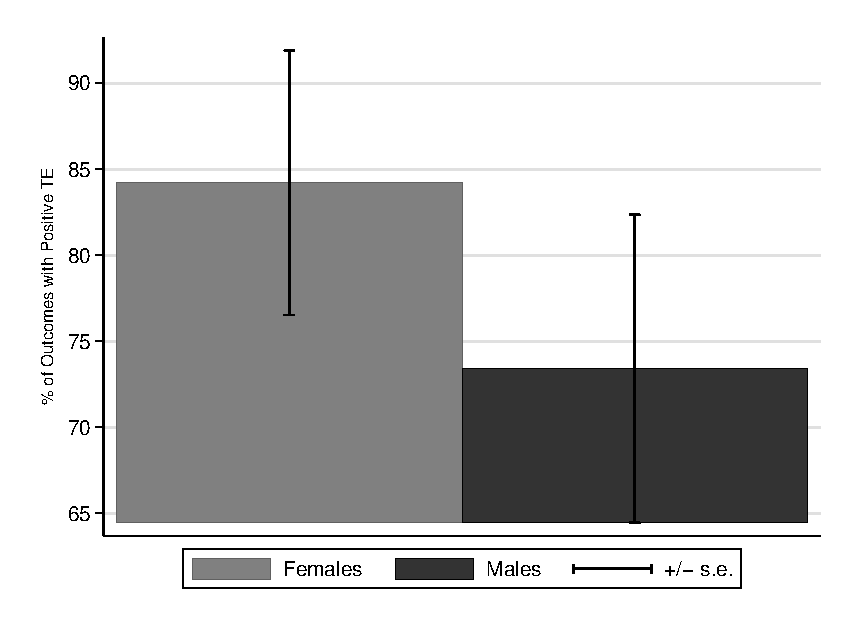
\includegraphics[width=\textwidth]{output/itt_noctrl_all.eps}
\end{subfigure}%
\begin{subfigure}[h]{0.4\textwidth}
	\centering
	\caption{Treatment vs. Next Best, Significant at 10\% Level} \label{fig:ppositive10}
		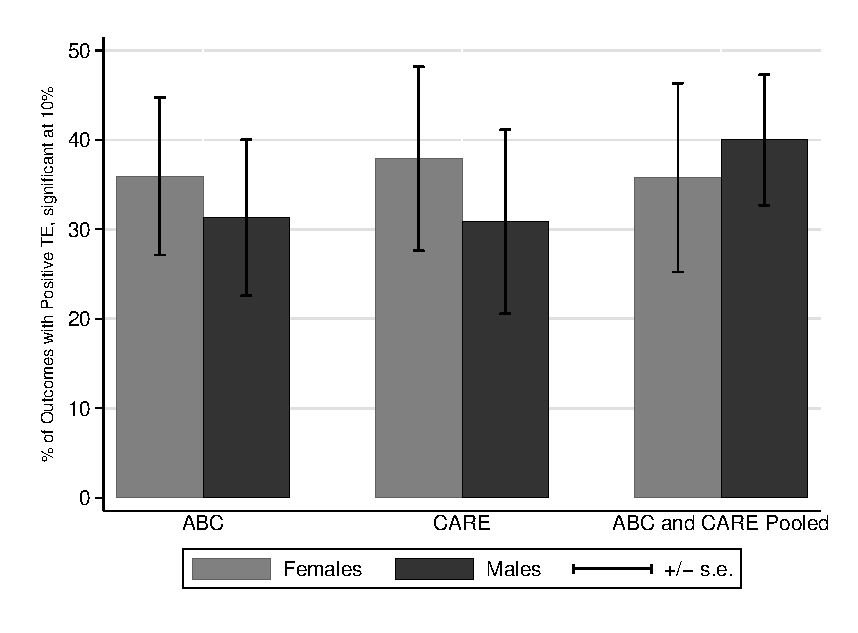
\includegraphics[width=\textwidth]{output/itt_noctrl_all_sig10.eps}
\end{subfigure}
\begin{subfigure}[h]{0.4\textwidth}
		\centering
		\caption{ Treatment vs. Stay at Home} \label{fig:ppositivehome}
		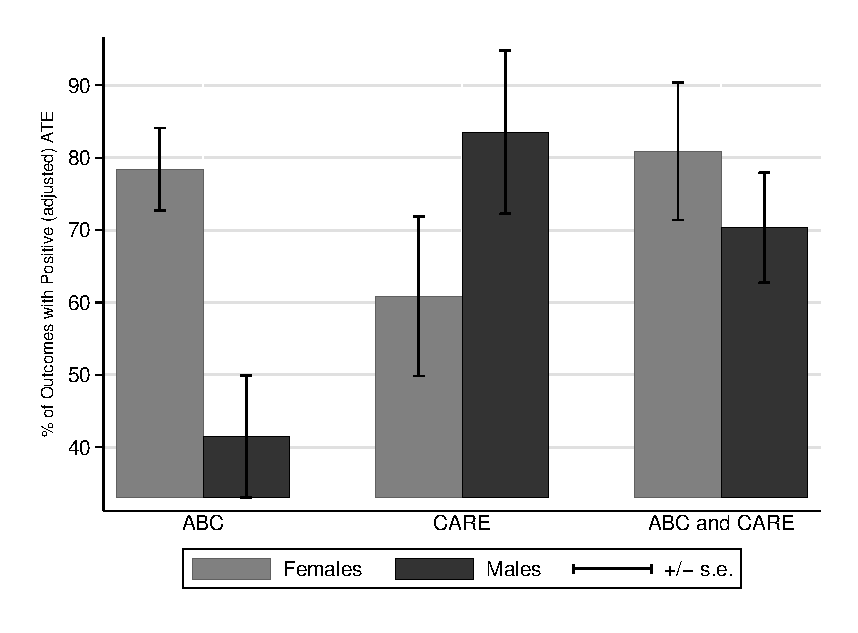
\includegraphics[width=\textwidth]{output/epan_ipw_p0_all.eps}
\end{subfigure}%
\begin{subfigure}[h]{0.4\textwidth}
	\centering
	\caption{Treatment vs. Alternative Preschool} \label{fig:ppositivealternative}
		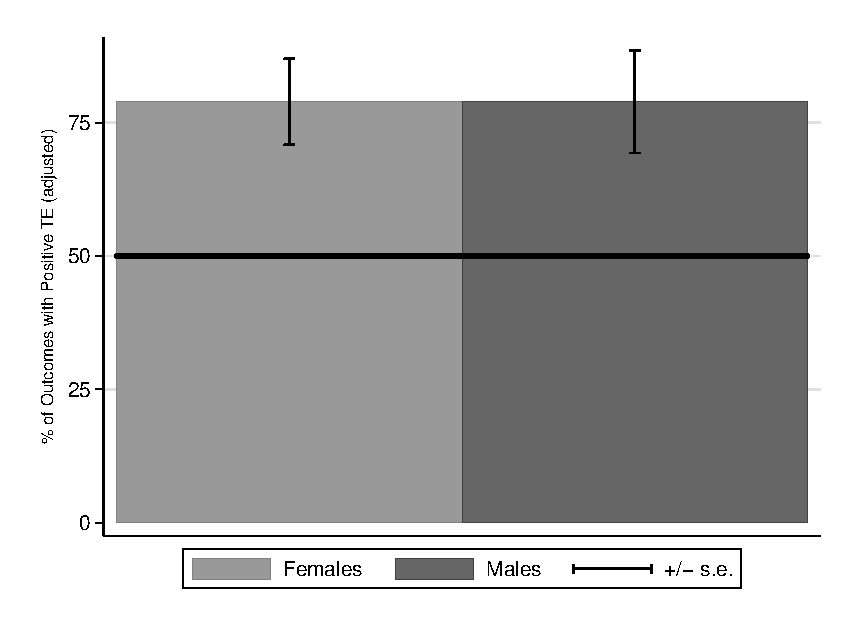
\includegraphics[width=\textwidth]{output/epan_ipw_p1_all.eps}
\end{subfigure}
\scriptsize \justify
Note: Panel (a) percentage of outcomes displaying a positive treatment effect, comparing treatment to next best. Panel (b) percentage of outcomes displaying a positive and statistically significant treatment effect (10\% significance level). Panel (c) displays the percentage of outcomes with a positive treatment effect, comparing treatment to staying at home. Panel (d) displays the percentage of outcomes with a positive treatment effect, comparing treatment to alternative childcare arrangements. Standard errors are based on the empirical bootstrap distribution. For Panel (b) we perform a ``double bootstrap'' procedure to first determine significant treatment effects at $10\%$ level and then calculate the standard error of the count.\\
\end{sidewaysfigure}

Finally, we present the estimates of the combining functions by outcome category. Figure~\ref{fig:cats-positive-significant} shows the estimated proportions that are statistically significantly positive at the 10\% level. Consistent with the treatment effects above, control-group females tend to do better in alternative childcare than at home. This is especially true for parenting measures, IQ, education, and employment. Control-group males, on the other hand, do better at home, with more positive treatment effects compared to low quality childcare.

\begin{figure}[H]
\centering
\caption{Proportion of Positively Impacted Outcomes by Category, ABC/CARE Males and Females}\label{fig:cats-positive-significant}
\begin{subfigure}[h]{0.7\textwidth}
	\centering
	\caption{Treatment vs. Stay at Home, Significant at 10\% Level}
		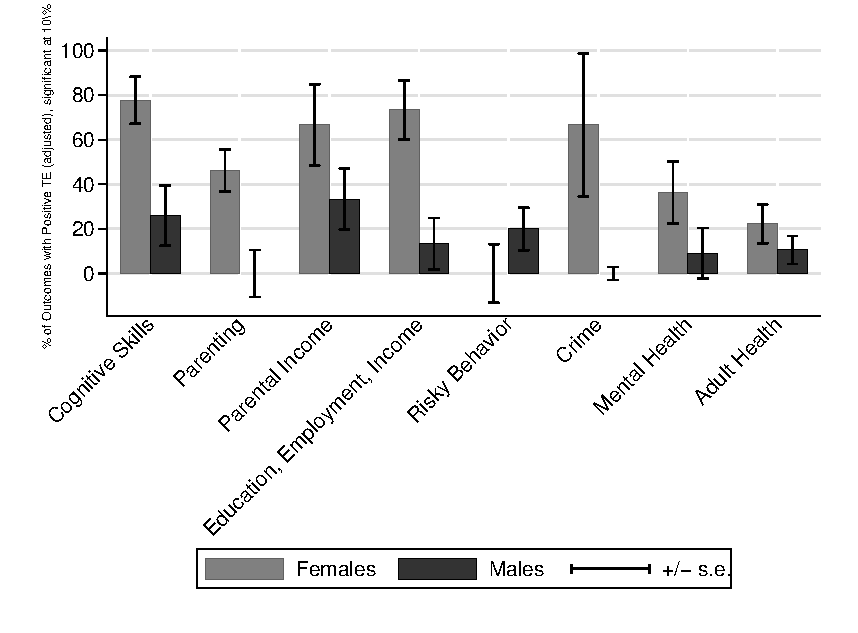
\includegraphics[width=\textwidth]{output/epan_ipw_p0_cats1_sig10.eps}
\end{subfigure}

\begin{subfigure}[h]{0.7\textwidth}
	\centering
	\caption{Treatment vs. Alternative Preschool, Significant at 10\% Level}
		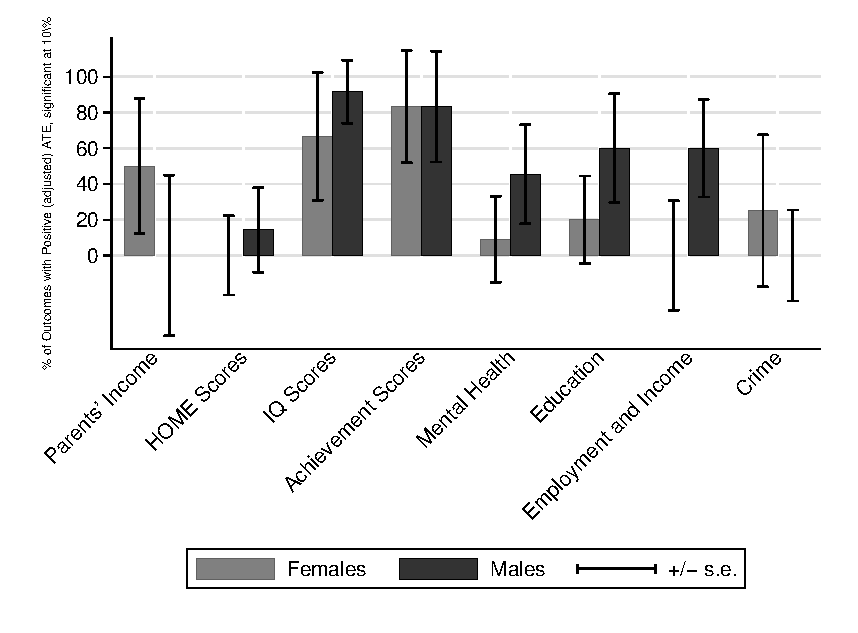
\includegraphics[width=\textwidth]{output/epan_ipw_p1_cats1_sig10.eps}
\end{subfigure}
\scriptsize \justify
Note: Panel (a) percentage of outcomes displaying a positive treatment effect, comparing treatment to next best. Panel (b) percentage of outcomes displaying a positive and statistically significant treatment effect (10\% significance level). Panel (c) displays the percentage of outcomes with a positive treatment effect, comparing treatment to staying at home. Panel (d) displays the percentage of outcomes with a positive treatment effect, comparing treatment to alternative childcare arrangements. Standard errors are based on the empirical bootstrap distribution. For Panel (b) we perform a ``double bootstrap'' procedure to first determine significant treatment effects at $10\%$ level and then calculate the standard error of the count.\\
\end{figure}



\section{Explaining Gender Differences}
\label{sec:gender-differences}

A better understanding of the counterfactual scenario that children would have faced if ABC/CARE were unavailable is useful in explaining the gender differences in the treatment effects. This requires us to identify the parameter in Equation~\eqref{eq:cont1}---the comparison between treatment and staying at home---and the parameter in Equation~\eqref{eq:cont2}---the analogous comparison to children who attended alternative preschools. These parameters are not identified by randomization into the treatment or control groups. The parents of the control-group children selected either to keep their children at home or take them to alternative preschools that were available when ABC/CARE was implemented. 

We rely on econometric methods for identification. In the main text, we rely on matching.\footnote{See \citet{Heckman_Ichimura_etal_1998_REStud} for a general discussion of the method, and an assessment of its practical implementation.} This method is practical in our case due to the small size of our samples. We show that the matching approach results in balanced samples (Table~\ref{tab:testing-matched-samples} in Appendix~\ref{app:matching-is-fun}). In Appendix~\ref{appendix:amethodology}, we show that instrumental-variable and control-function methods yield similar results but lack precision. In Appendix~\ref{appendix:results}, we discuss and document our choice of the matching variables, as well as other practical aspects of the implementation of this estimator.

Tables~\ref{table:massivealt} and~\ref{table:massivehome} provide analogous estimates to Table~\ref{table:massiveall}, using the different comparison groups (alternative preschool or stay at home). We argue that the $p$-values can be interpreted as magnitudes following \citet{Fisher_1935_Inference_JRSS}. In Table~\ref{table:massiveall}, with the full sample, the pattern of the $p$-values parallels that of the average effect sizes. In the comparison between the treatment group and those who attend alternative preschool, the  \citet{Rosenbaum_2005_Distribution_JRSS} $p$-value is significant for males more than for females. The exception to this is in education, in which the effect on females (0.332) is much larger than the effect of males (0.177). This pattern is reversed in the comparison between the treatment group and those who stayed at home. The exception to this is risky behavior, in which the effect on males (0.122) is much larger than the effect on females (0.054), even though the proportion of (significant) outcomes is the same. 

The intergenerational effect seen on the increase in parental income is strong across comparisons and genders. The effect size is larger in the comparison between treatment and those who stay at home, which is logical given that there are fewer labor market opportunities if the children stay at home. 

The effects on crime highlight that females were highly impacted by ABC/CARE, especially compared to those who attended alternative care. \citet{Garcia_Heckman_Leaf_etal_2017_Comp_CBA_Unpublished} find that even though the treatment effects on the crime outcomes are larger for women than for men, the men commit more socially expensive crimes. In the benefit/cost ratio that they compute, the effect of ABC/CARE on reducing individual male crimes is an important component. \citet{Garcia_etal_2019_ECE_IMHJ} discuss the crime results in more detail.

\begin{table}[!htpb]
\begin{threeparttable}
\caption{Combining Functions and Non-Parametric, Exact Tests, Treatment vs. Alternative} \label{table:massivealt}
\centering
 \begin{tabular}{l c c c c}
\toprule
 & Average & \% $ >0 $ & \% $ >0 $ , Significant & \citet{Rosenbaum_2005_Distribution_JRSS} \\
 & Effect Size & Treatment Effect & Treatment Effect & $ p $ -value \\
\midrule
\textbf{IQ} & & & & \\
\quad Females &  \textbf{    0.679} & \textbf{  100.000} & \textbf{  100.000} & .977 \\
\quad Males &  \textbf{    0.544} & \textbf{  100.000} & \textbf{  100.000} & .012 \\
\midrule
\textbf{Achievement} & & & & \\
\quad Females &  \textbf{    0.680} & \textbf{  100.000} & \textbf{  100.000} & .183 \\
\quad Males &  \textbf{    0.232} & \textbf{  100.000} & \textbf{   80.000} & .448 \\
\midrule
\textbf{Social-emotional} & & & & \\
\quad Females &  \textbf{    0.348} & \textbf{   85.714} & \textbf{   57.143} & .898 \\
\quad Males &  \textbf{    0.081} & \textbf{   64.286} & \textbf{   28.571} & .901 \\
\midrule
\textbf{Parental Income} & & & & \\
\quad Females &  \textbf{    0.211} & \textbf{  100.000} & \textbf{   60.000} & .052 \\
\quad Males &  \textbf{    0.299} & \textbf{  100.000} & \textbf{   60.000} & .061 \\
\midrule
\textbf{Parenting} & & & & \\
\quad Females &  \textbf{    0.173} & \textbf{  100.000} &    20.000 & .183 \\
\quad Males &     -0.003 & \textbf{   60.000} &     0.000 & .061 \\
\midrule
\textbf{Education} & & & & \\
\quad Females &  \textbf{    0.332} & \textbf{   83.333} & \textbf{   83.333} & .052 \\
\quad Males &  \textbf{    0.177} & \textbf{   83.333} & \textbf{   33.333} & .448 \\
\midrule
\textbf{Employment} & & & & \\
\quad Females &  \textbf{    0.164} & \textbf{  100.000} & \textbf{   50.000} & .429 \\
\quad Males &  \textbf{    0.491} & \textbf{  100.000} & \textbf{   50.000} & .448 \\
\midrule
\textbf{Crime} & & & & \\
\quad Females &  \textbf{    0.334} & \textbf{  100.000} & \textbf{  100.000} & .898 \\
\quad Males &     -0.322 & \textbf{   33.333} &     0.000 & .448 \\
\midrule
\textbf{Risky Behavior} & & & & \\
\quad Females &  \textbf{    0.140} & \textbf{  100.000} &     0.000 & .708 \\
\quad Males &     -0.050 & \textbf{   25.000} & \textbf{   25.000} & .448 \\
\midrule
\textbf{Health} & & & & \\
\quad Females &      0.093 & \textbf{   68.750} & \textbf{   31.250} & .835 \\
\quad Males &      0.080 & \textbf{   56.250} & \textbf{   31.250} & 0 \\
\bottomrule
\end{tabular}
% This file generated by: /scripts/abccare/genderdifferences/abccare-gdiff-raw-rosenbaum-table-big.do
 
\begin{tablenotes}
\footnotesize
\item \footnotesize \textbf{Note:} This table displays summaries of treatment effects by outcome category and gender. The comparison group is the control-group children who attend alternatives. The panels contains statistics calculated using outcomes grouped by category. The average effect size is calculated by averaging over the effect size of the outcomes in the outcome category. The effect sizes of the individual outcomes are calculated by dividing the coefficient by the standard deviation of the control group. We test these three statistics bootstrapped $p$-values. For the proportion of outcomes that are positive and significant, we do a ``double bootstrap'' procedure. The null hypothesis for the effect sizes is that they are 0. The null hypothesis for the proportion of outcomes that are (significantly) positive is that they are (10\%) 50\%. Bolded statistics are significant at the 10\% level. The \citet{Rosenbaum_2005_Distribution_JRSS} $p$-value originates from a test where the null is a common joint distribution of the variables in each category. Statistics significant at the $0.10$ level are bolded.
\end{tablenotes}
\end{threeparttable}
\end{table}

\begin{table}[!htpb]
\begin{threeparttable}
\caption{Combining Functions and Non-Parametric, Exact Tests, Treatment vs. Home Care} \label{table:massivehome}
\centering
 \begin{tabular}{l c c c c}
\toprule
 & Average & \% $ >0 $ & \% $ >0 $ , Significant & \citet{Rosenbaum_2005_Distribution_JRSS} \\
 & Effect Size & Treatment Effect & Treatment Effect & $ p $ -value \\
\midrule
\textbf{IQ} & & & & \\
\quad Females &  \textbf{    0.703} & \textbf{  100.000} & \textbf{  100.000} & .061 \\
\quad Males &  \textbf{    0.829} & \textbf{  100.000} & \textbf{  100.000} & .02 \\
\midrule
\textbf{Achievement} & & & & \\
\quad Females &  \textbf{    0.397} & \textbf{  100.000} & \textbf{   80.000} & .414 \\
\quad Males &  \textbf{    0.446} & \textbf{  100.000} & \textbf{   80.000} & .823 \\
\midrule
\textbf{Social-emotional} & & & & \\
\quad Females &  \textbf{    0.221} & \textbf{   71.429} & \textbf{   64.286} & .414 \\
\quad Males &  \textbf{    0.237} & \textbf{   92.857} & \textbf{   64.286} & .394 \\
\midrule
\textbf{Parental Income} & & & & \\
\quad Females &  \textbf{    0.336} & \textbf{  100.000} & \textbf{   80.000} & .061 \\
\quad Males &  \textbf{    0.460} & \textbf{  100.000} & \textbf{  100.000} & .053 \\
\midrule
\textbf{Parenting} & & & & \\
\quad Females &  \textbf{    0.255} & \textbf{  100.000} & \textbf{   80.000} & .414 \\
\quad Males &  \textbf{    0.290} & \textbf{  100.000} & \textbf{   80.000} & .823 \\
\midrule
\textbf{Education} & & & & \\
\quad Females &  \textbf{    0.292} & \textbf{   83.333} & \textbf{   50.000} & .061 \\
\quad Males &  \textbf{    0.311} & \textbf{   83.333} & \textbf{   50.000} & .394 \\
\midrule
\textbf{Employment} & & & & \\
\quad Females &  \textbf{    0.424} & \textbf{  100.000} & \textbf{  100.000} & .867 \\
\quad Males &  \textbf{    0.389} & \textbf{  100.000} & \textbf{  100.000} & .394 \\
\midrule
\textbf{Crime} & & & & \\
\quad Females &     -0.278 & \textbf{   33.333} &     0.000 & .024 \\
\quad Males &      0.112 & \textbf{   66.667} & \textbf{   66.667} & .394 \\
\midrule
\textbf{Risky Behavior} & & & & \\
\quad Females &      0.054 & \textbf{   50.000} & \textbf{   25.000} & .414 \\
\quad Males &  \textbf{    0.122} & \textbf{   50.000} & \textbf{   25.000} & .002 \\
\midrule
\textbf{Health} & & & & \\
\quad Females &      0.005 & \textbf{   56.250} & \textbf{   25.000} & .002 \\
\quad Males &  \textbf{    0.075} & \textbf{   80.000} & \textbf{   46.667} & .02 \\
\bottomrule
\end{tabular}
% This file generated by: /scripts/abccare/genderdifferences/abccare-gdiff-raw-rosenbaum-table-big.do
 
\begin{tablenotes}
\footnotesize
\item  \footnotesize \textbf{Note:} This table displays summaries of treatment effects by outcome category and gender. The comparison group is the control-group children who stay at home.The panels contains statistics calculated using outcomes grouped by category. The average effect size is calculated by averaging over the effect size of the outcomes in the outcome category. The effect sizes of the individual outcomes are calculated by dividing the coefficient by the standard deviation of the control group. We test these three statistics bootstrapped $p$-values. For the proportion of outcomes that are positive and significant, we do a ``double bootstrap'' procedure. The null hypothesis for the effect sizes is that they are 0. The null hypothesis for the proportion of outcomes that are (significantly) positive is that they are (10\%) 50\%. Bolded statistics are significant at the 10\% level. The \citet{Rosenbaum_2005_Distribution_JRSS} $p$-value originates from a test where the null is a common joint distribution of the variables in each category. Statistics significant at the $0.10$ level are bolded.
\end{tablenotes}
\end{threeparttable}
\end{table}

\begin{sidewaysfigure}[!htpb]
\centering
\caption{Gender and Baseline Socioeconomic Disadvantage in the Control Group} \label{figure:socdis}
\begin{subfigure}[h]{0.4\textwidth}
	\centering
	\caption{Take-up of Alternatives by Gender} \label{figure:altgender}
	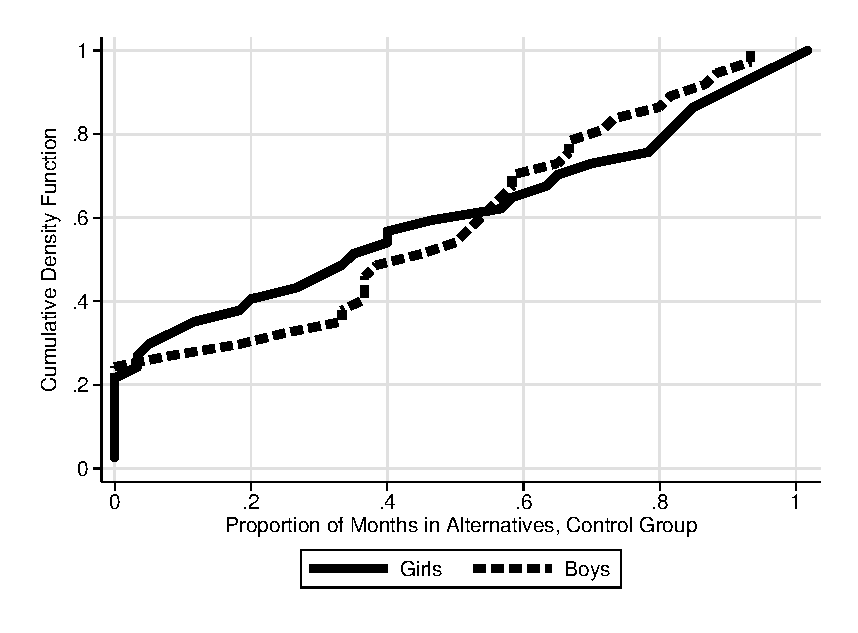
\includegraphics[width=\textwidth]{output/abccare_controlcontamination_boysgirls}
\end{subfigure}%
\begin{subfigure}[h]{0.4\textwidth}
	\centering
	\caption{Socioeconomic Disadvantage by Gender} \label{figure:disadgender}
	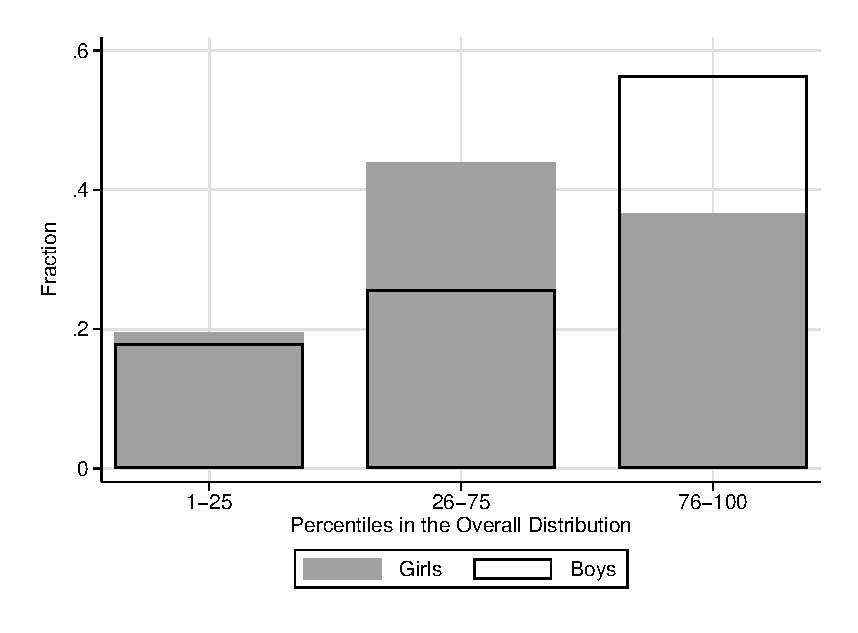
\includegraphics[width=\textwidth]{output/factorbase_girlsboyscompare}
\end{subfigure}
\begin{subfigure}[h]{0.4\textwidth}
	\centering
	\caption{Disadvantage by Take-up of Alternatives, Girls} \label{figure:disadgirls}
	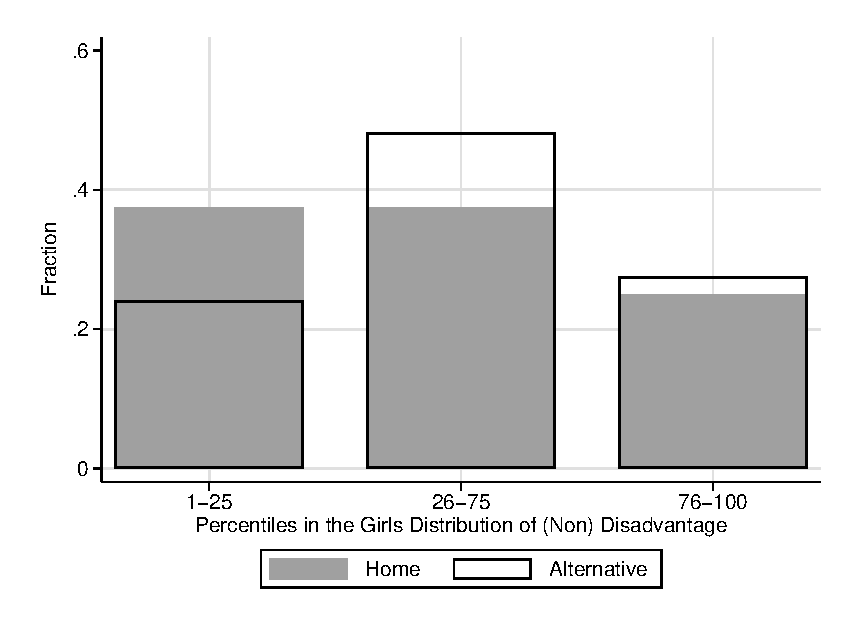
\includegraphics[width=\textwidth]{output/factorbase_wgirlscompare}
\end{subfigure}%
\begin{subfigure}[h]{0.4\textwidth}
	\centering
	\caption{Disadvantage by Take-up of Alternatives, Boys} \label{figure:disadboys}
	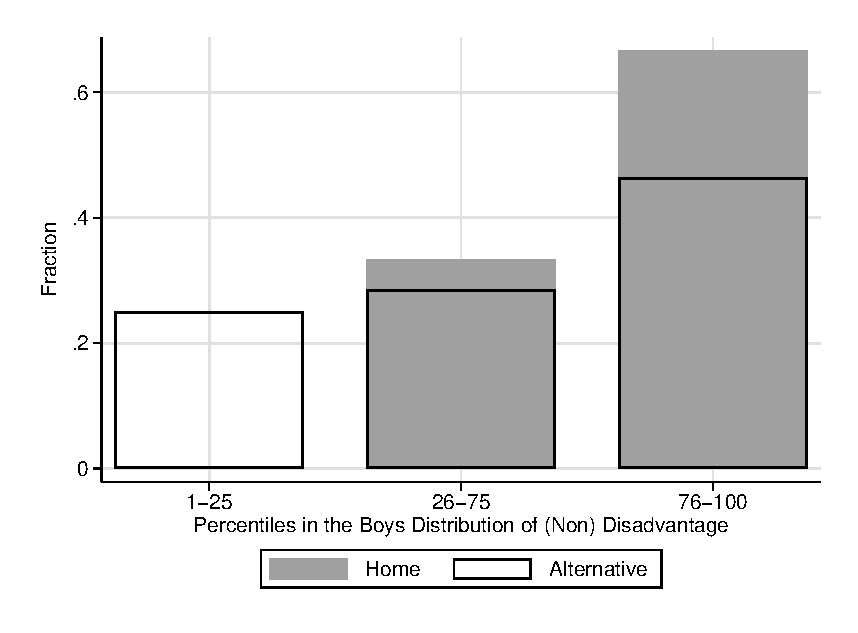
\includegraphics[width=\textwidth]{output/factorbase_wboyscompare}
\end{subfigure}
\footnotesize
\justify
\textbf{Note:} Panel (a) displays the cumulative distribution function of enrollment in alternatives by gender. Panel (b) displays how girls and boys separately fit into the overall (girls and boys pooled) distribution of socioeconomic disadvantage. Panel (c) displays how girls who did not enroll and girls who enrolled in alternatives fit into the overall female distribution of socioeconomic disadvantage. Panel (d) is analogous to Panel (c) for boys. Our measure of socioeconomic disadvantage is a latent of the following variables: Mother's age, education, IQ, marital status, and employment, as well as number of siblings and father's presence at home.
\end{sidewaysfigure}

The difference in the comparison of treatment to staying at home and alternative preschools suggests that boys and girls faced different situations of socio-economic disadvantaged at home. Figure~\ref{figure:socdis} investigates this. We start by noting that take-up of alternatives does not differ by gender (Panel~\ref{figure:altgender}). What does differ by gender is socioeconomic disadvantage. We create a latent measure of socioeconomic disadvantage at baseline using the following variables: Mother's age, education, IQ, marital status, and employment, as well as number of children and father's presence at home. We assess how girls and boys fit into the overall distribution of this latent in the control group. Boys are disproportionately more advantaged than girls (Panel~\ref{figure:disadgender}).\footnote{Note that this measure is based on baseline characteristics, so this result holds for the treatment group.} Because girls' families were more resource constrained if compared to their male counterparts, girls in the control group were taken care of in a more disadvantaged environment or went to lower-quality preschools. Thus, they benefited more than boys if compared to the next best alternative as perceived by their parents, as documented in Section~\ref{sec:treatment-effects}.


\begin{table}[!htpb]
\begin{threeparttable}
\caption{Gender and Baseline Socioeconomic Disadvantage in the Control Group, Tests} \label{table:disadtests}
\centering 
\begin{tabularx}{16.5cm}{XcX}
& \begin{tabular}{cccc}
\toprule
Males vs. Females & & \mc{2}{c}{Alt. vs. Home} \\
\cmidrule(lr){1-2} \cmidrule(lr){3-4}
Control Group & & Males & Females \\
\midrule
\textbf{0.007} & & \textbf{0.006} & 0.110 \\
\bottomrule
\end{tabular}

% Control, males vs. females: distance between: factor of m_age_base, m_ed_base, m_iq_base, hh_sibs_base, hrabc_index

% Alt. vs home: factor of m_age_base, m_ed_base, m_iq_base, hh_sibs_base, hrabc_index & 
\end{tabularx}
\begin{tablenotes}
\footnotesize
\item \textbf{Note:} This table presents the null of a common joint distribution of the variables composing our measure of socioeconomic disadvantage (mother's age, education, IQ, marital status, and employment, as well as number of siblings and father's presence at home) between males and females in the control group and between children who attended  alternative preschool and who stayed at home (within control-group boys or within control-group girls). The $p$-values follow \citet{Rosenbaum_2005_Distribution_JRSS}. Under the null hypothesis, the pairs with the closest distance in disadvantage would be comprised of one male and one female (for the comparison of males vs. females). Rejecting the null implies that the distributions are significantly different. Statistics significant at the $0.10$ level are bolded.
\end{tablenotes}
\end{threeparttable}
\end{table}

We formally test the difference in disadvantage across boys and girls in Table~\ref{table:disadtests}. We reject the null of a common joint distribution of the variables composing our measure of socioeconomic disadvantage across girls and boys (at baseline). In Panels~\ref{figure:disadgirls} and~\ref{figure:disadboys} of Figure~\ref{figure:socdis}, we further dissect socioeconomic disadvantage within genders, and provide the corresponding tests in Table~\ref{table:disadtests}. 


Parents of more advantaged girls are more likely to send their daughters to alternative preschools. Parents of more advantaged boys are more likely to send keep their sons at home. This provides an explanation why girls benefited more from treatment if compared to staying at home, which would be a more disadvantaged environment if compared to the male environments. Boys benefited more from treatment if compared to attending alternatives given that their parents plausibly sent them to lower-quality alternatives due to a lack of resources or the alternatives were worse complements to home learning environments. 













\section{Summary and Conclusions}
\label{sec:conclusion}
\textbf{[JJH: I will rewrite when we resolve. Section 5 is a mess. The paper falls apart in Figure 3.] [JLG: I believe that the first two paragraphs much better summarize the paper, and the third paragraph is not relevant anymore and the evidence is not as strong as to support that claim.]}

This paper examines gender differences in the impacts of treatment of an influential early childhood program targeted to disadvantaged children. Upon the impracticality of analyzing the dozens of outcomes available to evaluate the program one at the time and the need to avoid cherry-picking outcomes with significant treatment effects, we propose parametric and non-parametric tests to aggregate and summarize treatment effects. We document that girls benefit more than boys. 

The source of the gender difference is worse control-group conditions for girls resulting from more severe socio-economic disadvantage at baseline. Fathers of sons are more likely to support spouses than fathers of daughters. Boys are more advantaged, with the more advantaged boys being more likely to stay at home. This explains why the effects are larger for males in comparison to alternative care than in comparison to staying at home. For girls, the difference in advantage between the different counterfactual scenarios is not as stark. The effects are larger in general for girls in comparison to staying at home than in comparison to alternative care, but the statistical tests are not as robust as for boys.

Our analysis sounds a cautionary note about the value of early childcare programs. In the past decade, many politicians and pundits have warmly embraced early childhood programs as solutions for reducing inequality and promoting social mobility. Little attention has been paid to the quality of those programs. \cite{Garcia_Heckman_Leaf_etal_2017_Comp_CBA_Unpublished} show that they have a high economic rate of return. Even though we find that females benefit more in terms of effect sizes and in the number of statistically significant treatment effects than do males, after weighing for the social benefits of reduced crime and improved health, education, and employment, the social return is higher for males than females.

\clearpage

\singlespacing
\bibliography{heckman}
\bibliographystyle{chicago}

\end{document}
